\documentclass[a4paper, 12pt, notitlepage]{article} % Style du document
\usepackage[margin=1.3in]{geometry} % Petite marge
\usepackage[francais]{babel} % Langue du document

\usepackage[utf8]{inputenc} % Codage du fichier
\usepackage[T1]{fontenc} % Pour bien gérer les accents

\usepackage{cmbright} % Police utilisée

\usepackage{graphicx} % Pour pouvoir placer des images

\usepackage{verbatim}

\usepackage[french, onelanguage, slide, boxruled, lined, longend, linesnumbered]{algorithm2e} % Pour écrire du pseudo code

\usepackage{xspace} % Gère les espaces après les commandes
\usepackage{hyperref} % Pour ajouter des liens dans le document
\usepackage[french]{varioref}
\hypersetup{
  colorlinks, 
  linktoc=all, 
  citecolor=black, 
  linkcolor=black, 
  urlcolor=black, 
  pageanchor=false
}

% Pour pouvoir utiliser des couleurs
\usepackage{xcolor}
% Définition des couleurs du thème Paris-Sud (couleurs du logo)
\definecolor{bleuPS}{HTML}{004870}
\definecolor{vertPS}{HTML}{84b818}
\definecolor{grisPS}{HTML}{6b6c6e}

\setlength{\parskip}{0.6ex} % Ajoute un peu d'espace entre les paragraphes
\usepackage{titlesec} % Contre le changement d'espace dans les sections
\titlespacing*{\section}{0pt}{2.5ex}{1 ex}
\titlespacing*{\subsection}{0pt}{2.5ex}{1 ex}

\usepackage[ampersand]{easylist} % Pour faire des liste facilement
\newcommand\itemizeTrait{\ListProperties(Space=0ex, Space*=0ex, Style*=-- )} % Liste simple
\newcommand\itemizePuce{\ListProperties(Space=0ex, Space*=0ex, Style*=$\bullet$\ , Style2*=$\bullet$\ )} % Liste à puce

\usepackage{microtype} % Pour un texte bien mieux justifié

% Pour ajouter des pieds de pages
\usepackage{fancyhdr}
\pagestyle{fancy}
% Création des pieds de pages
\fancyhf{}
\lfoot{\textcolor{grisPS}{BestProjetGLA}}
\cfoot{\thepage}
\rfoot{\textcolor{grisPS}{Année 2016-2017 L3 Informatique}}
\renewcommand{\headrulewidth}{0pt}
\renewcommand{\footrulewidth}{1pt}
    
% Changement de couleurs des sections, sous-sections etc.
\usepackage{sectsty}
\sectionfont{\color{bleuPS}}
\subsectionfont{\color{vertPS}}
\subsubsectionfont{\color{grisPS}}

% Juste pour mettre du texte random en attendant d'écrire
\usepackage{lipsum}

% Spécifie le dossier des images
\usepackage{subfig}
\graphicspath{{Images/}}
\usepackage{caption}
\DeclareCaptionType{maquetteFig}[Maquette][Table des maquettes]
\DeclareCaptionType{umlFig}[Diagramme UML][Table des diagrammes UML]

\usepackage{longtable, lscape}

\begin{document}

% Création de la page de garde
\begin{titlepage}
	\centering
	
\includegraphics[width=0.2\textwidth]{LogoUPSUD_ParisSaclay.jpg}\par\vspace{1cm}
	{\scshape\large Projet Génie Logiciel Avancé L3 \par}
	\vspace{1cm}
	{\scshape\LARGE Cahier de conception\par}
	\vspace{1cm}
	{\huge\bfseries Assistant événementiel de sorties\par}
	\vspace{2cm}
	{\large CHOUKCHOU BRAHAM Abbes \\
					NDIAYE Thierno Ismaila\\
					VACHAUDEZ Cédric\par}
	\vfill
	Professeurs :\par NGUYEN VAN Hai\\FAISSOLE Florian
	\vfill
	{\large Année 2016-2017 L3 Informatique\par\par}
\end{titlepage}

% Table des matières non numéroté et sans pied de page
\pagenumbering{gobble}
{
\setlength{\parskip}{0 ex}
\tableofcontents
\thispagestyle{empty}
\newpage

\listoffigures
\thispagestyle{empty}
}
\newpage
\pagenumbering{arabic}


\section{Introduction}
Le but de ce document est de présenter l'architecture de l'application BestProjetGLA de manière plus détaillée que le cahier des charges ainsi que les tests qui devront être menés.

Cette application a pour but d'offrir à ses utilisateurs un moyen automatisé et simple pour organiser une soirée. Après avoir donné les participants, la date, les contraintes et la suite d'étapes que la soirée devra comprendre, l'application se chargera de trouver un parcours passant par toutes ces étapes en respectant les contraintes (qu'il s’agisse des horaires ou de contraintes données par l'utilisateur).

\subsection{Caractéristiques du système visé}
L'application devant fonctionner sur les téléphones Android en version 4.1.2 minimum, il faudra donc utiliser l'API 16.
Le langage de programmation est très proche de Java et possède toutes ses caractéristiques, notamment la programmation orientée objet.

Les ressources sont très limitées. Il faudra donc consommer le moins de mémoire RAM et physique possible, limiter la demande en bande passante, et prendre en compte l'instabilité du réseau mobile 3G/4G.
L'application devra aussi avoir une interface fluide et agréable avec un contenu adapté aux différents formats d'écrans.

\subsection{Dépendances}
Les APIs Google Places et Google Maps seront nécessaires car exploitées pour trouver les différentes étapes de la sortie, pour afficher une carte et transformer les adresses en coordonnées GPS (latitude,longitude...).

Aussi, l'utilisation d'une base de données interne sera primordiale pour sauvegarder et manipuler nos données et faire tourner l'application en mode déconnecté. Android implémentant depuis toujours SQLite, ce sera donc elle qui sera utilisée.
\clearpage



\section{Structure globale}
Les différentes actions possibles de l’utilisateur ont été représentées par le diagramme \ref{fig:EtatTrans}, tandis que les classes dont sera constituée l'application sont représentées dans le diagramme \ref{fig:Classes}.

\vfill
\begin{figure}[!htb]
    \centering
    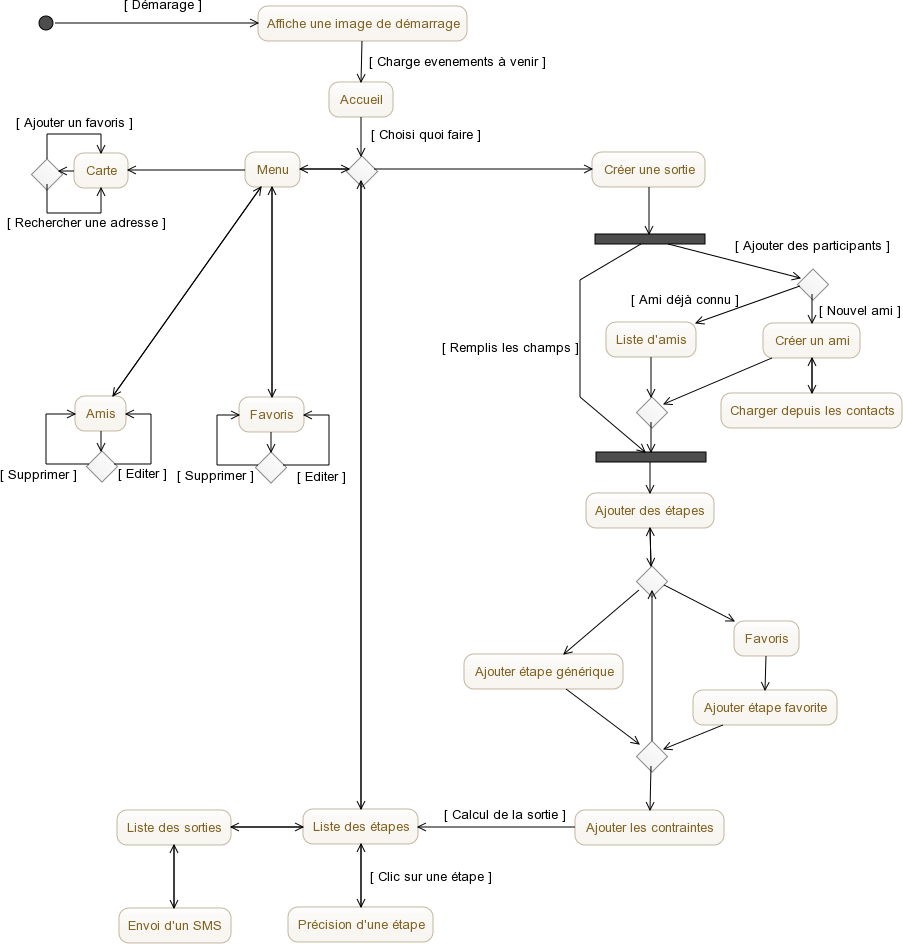
\includegraphics[width=1\textwidth]{Diagramme_d_etat.png}
    \caption[Diagramme états-transitions]{Diagramme états-transitions représentant tous les déplacements possibles de l'utilisateur au sein de l'application}
    \label{fig:EtatTrans}
\end{figure}
\vfill

\begin{figure}[!htb]
    \centering
    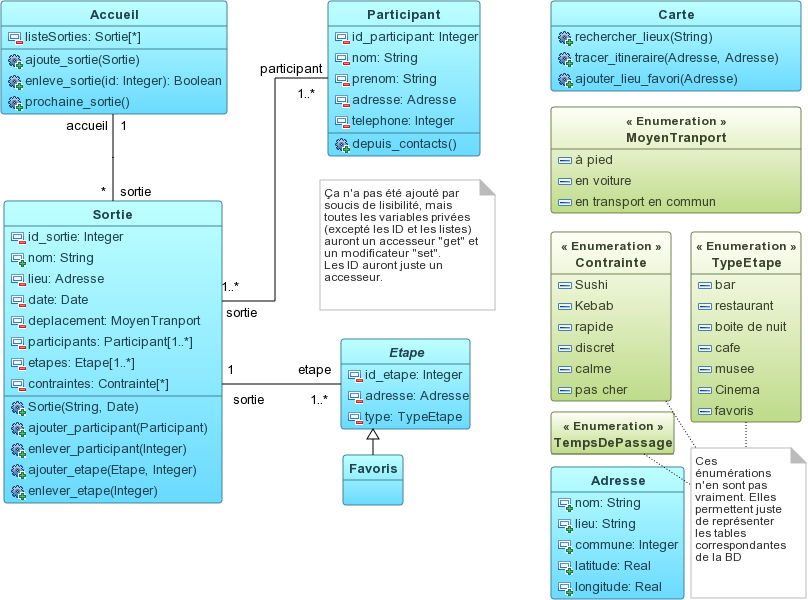
\includegraphics[width=1\textwidth]{Diagramme_de_classe_principal.png}
    \caption[Diagramme des classes principales]{Diagramme présentant les classes (et leurs relations) telles qu'elles seront implémentées dans notre application}
    \label{fig:Classes}
\end{figure}
\clearpage

\subsection{Base de données}
La base de données sera nécessaire pour stocker en local toutes les informations qu'il serait utile de garder. Cela peut concerner les favoris, les différentes soirées déjà organisées, mais aussi pour exploiter plus proprement d'autres données telle que la liste des étapes possibles où leur durée.

Sa structure sera assez proche de celle des classes afin de rendre sa manipulation la plus logique possible.

\vfill
\begin{figure}[!htb]
    \centering
    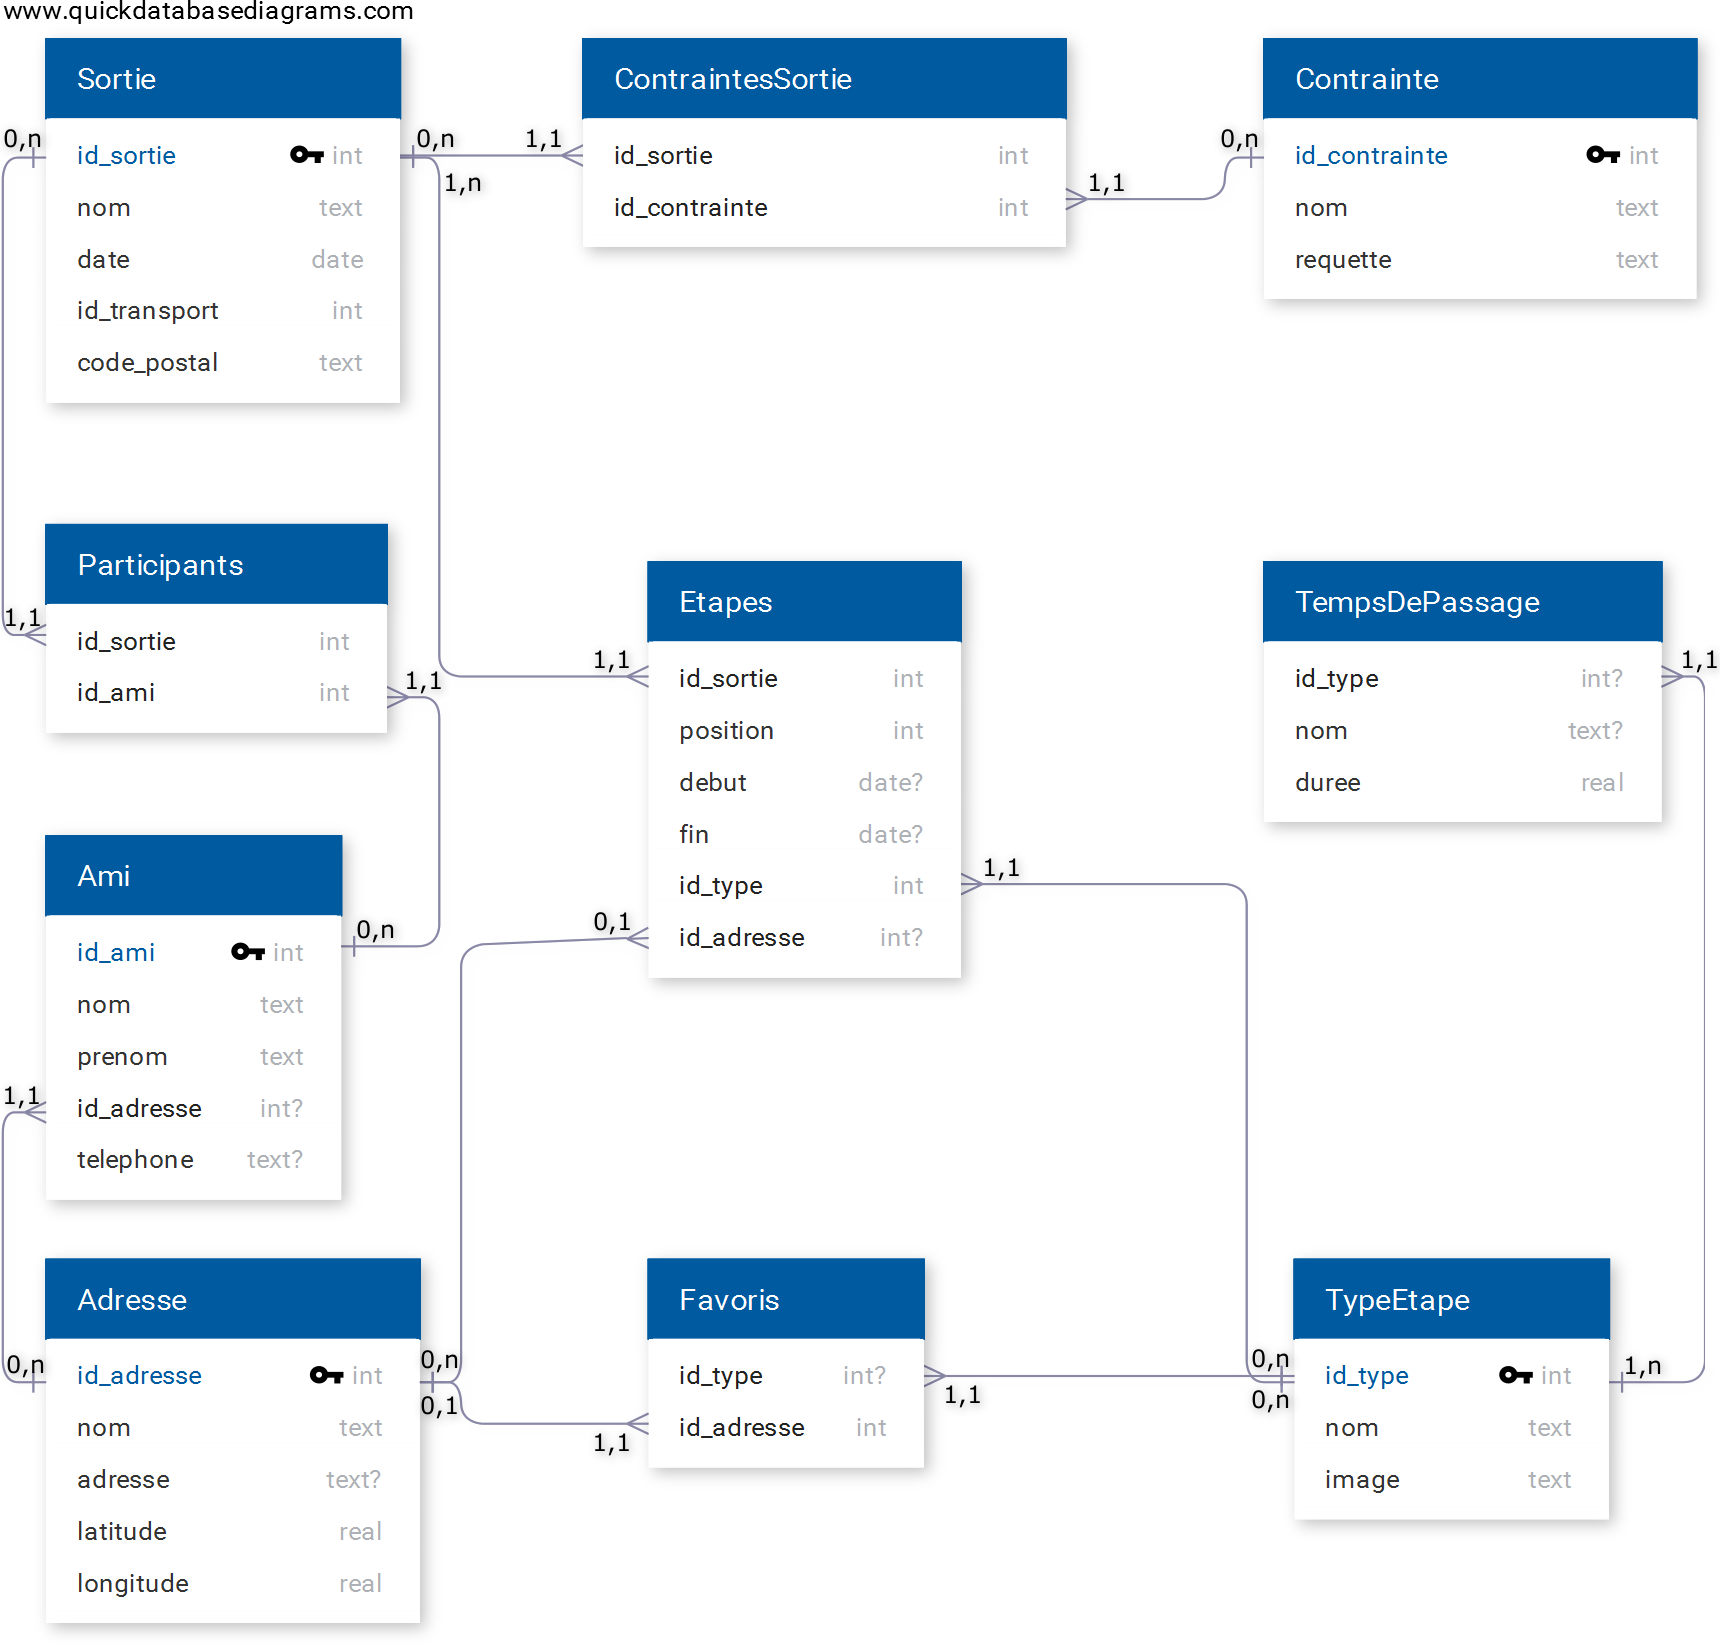
\includegraphics[width=1\textwidth]{DB_cardinal.png}
    \caption[Diagramme entités-relations]{Diagramme entités-relations présentant la structure de la base de données}
    \label{fig:BD}
\end{figure}
\vfill
\clearpage



\section{Démarrage}
Le démarrage de l'application est assez sobre : une image s'affichera avec son nom et son logo, permettant de faire patienter l'utilisateur le temps qu'elle s’initialise et charge les futures sorties (s'il y en a) dans la base de données.
Cette partie est présentée dans le diagramme \ref{fig:Accueil}.

On affichera ensuite l'accueil (interface \ref{interface:Accueil}) qui donnera un aperçu des soirées à venir (ou en cours) ainsi qu'un accès rapide à toutes les fonctions de l’application à l'aide du menu (interface \ref{interface:MenuAccueil}).

\vfill
\begin{figure}[!htb]
    \centering
    \hfill
    \subfloat[Accueil de l'application]{
    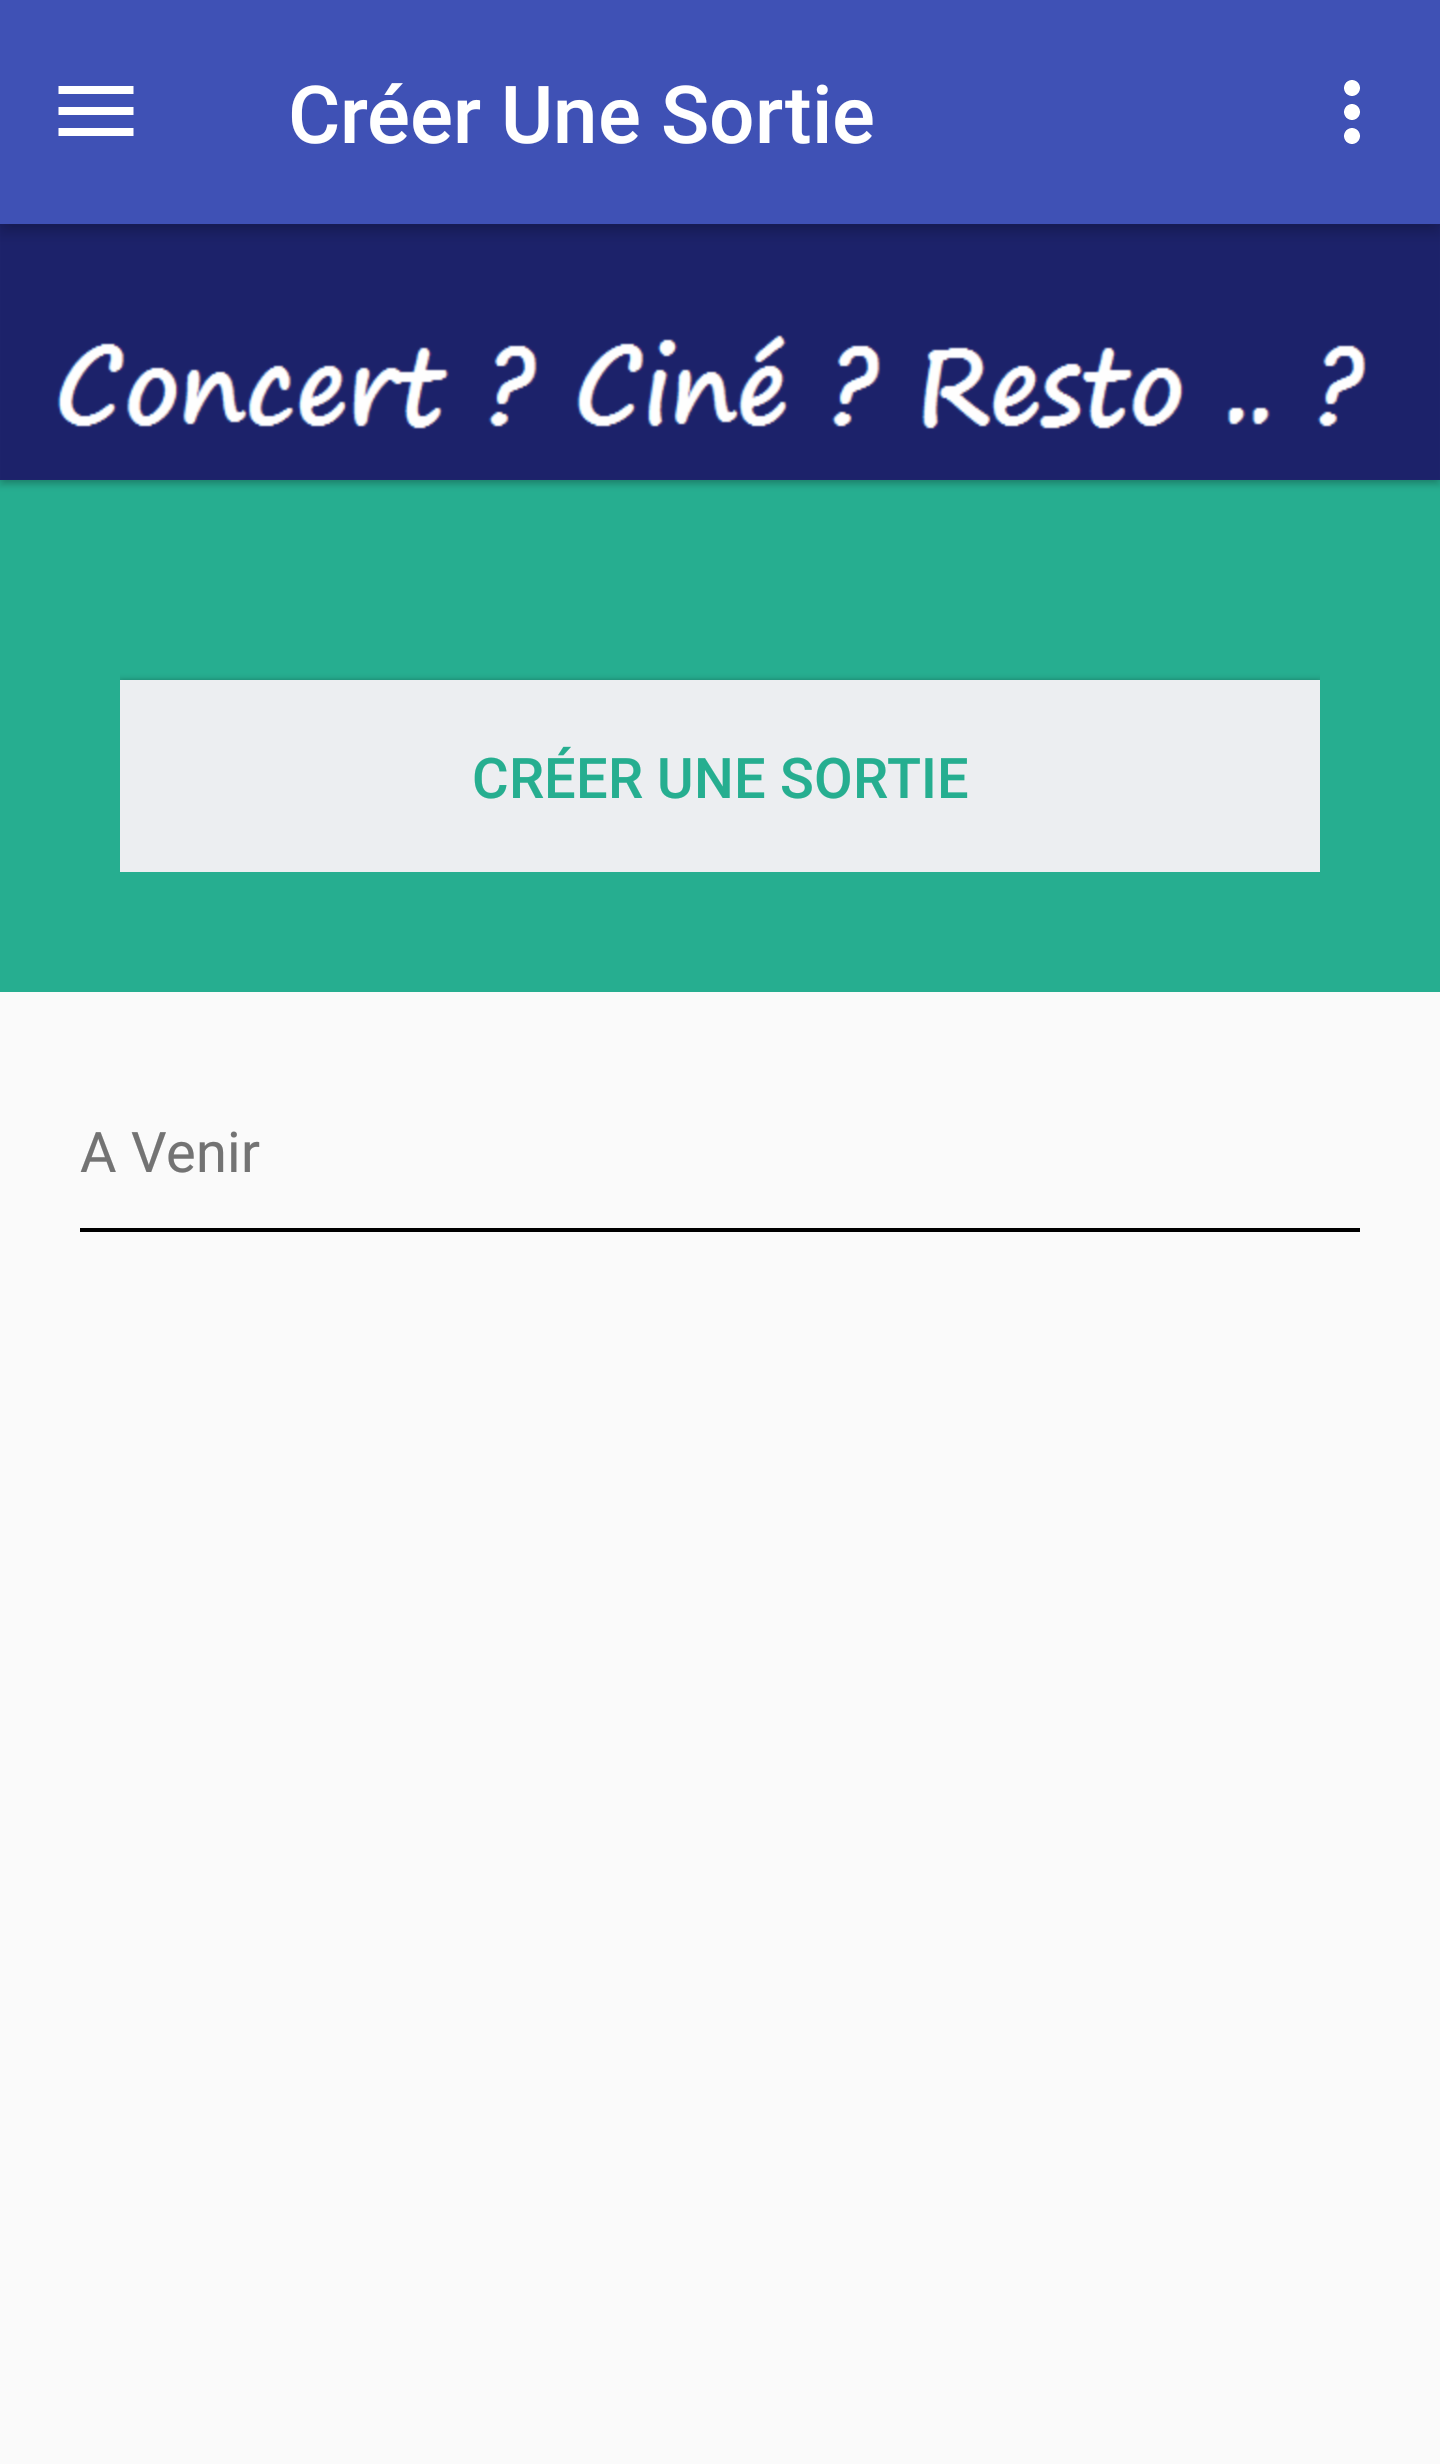
\includegraphics[height=0.4\textheight]{Interface_Accueil.png}
    \label{interface:Accueil}}
    \hfill
    \subfloat[Menu de l'application]{
    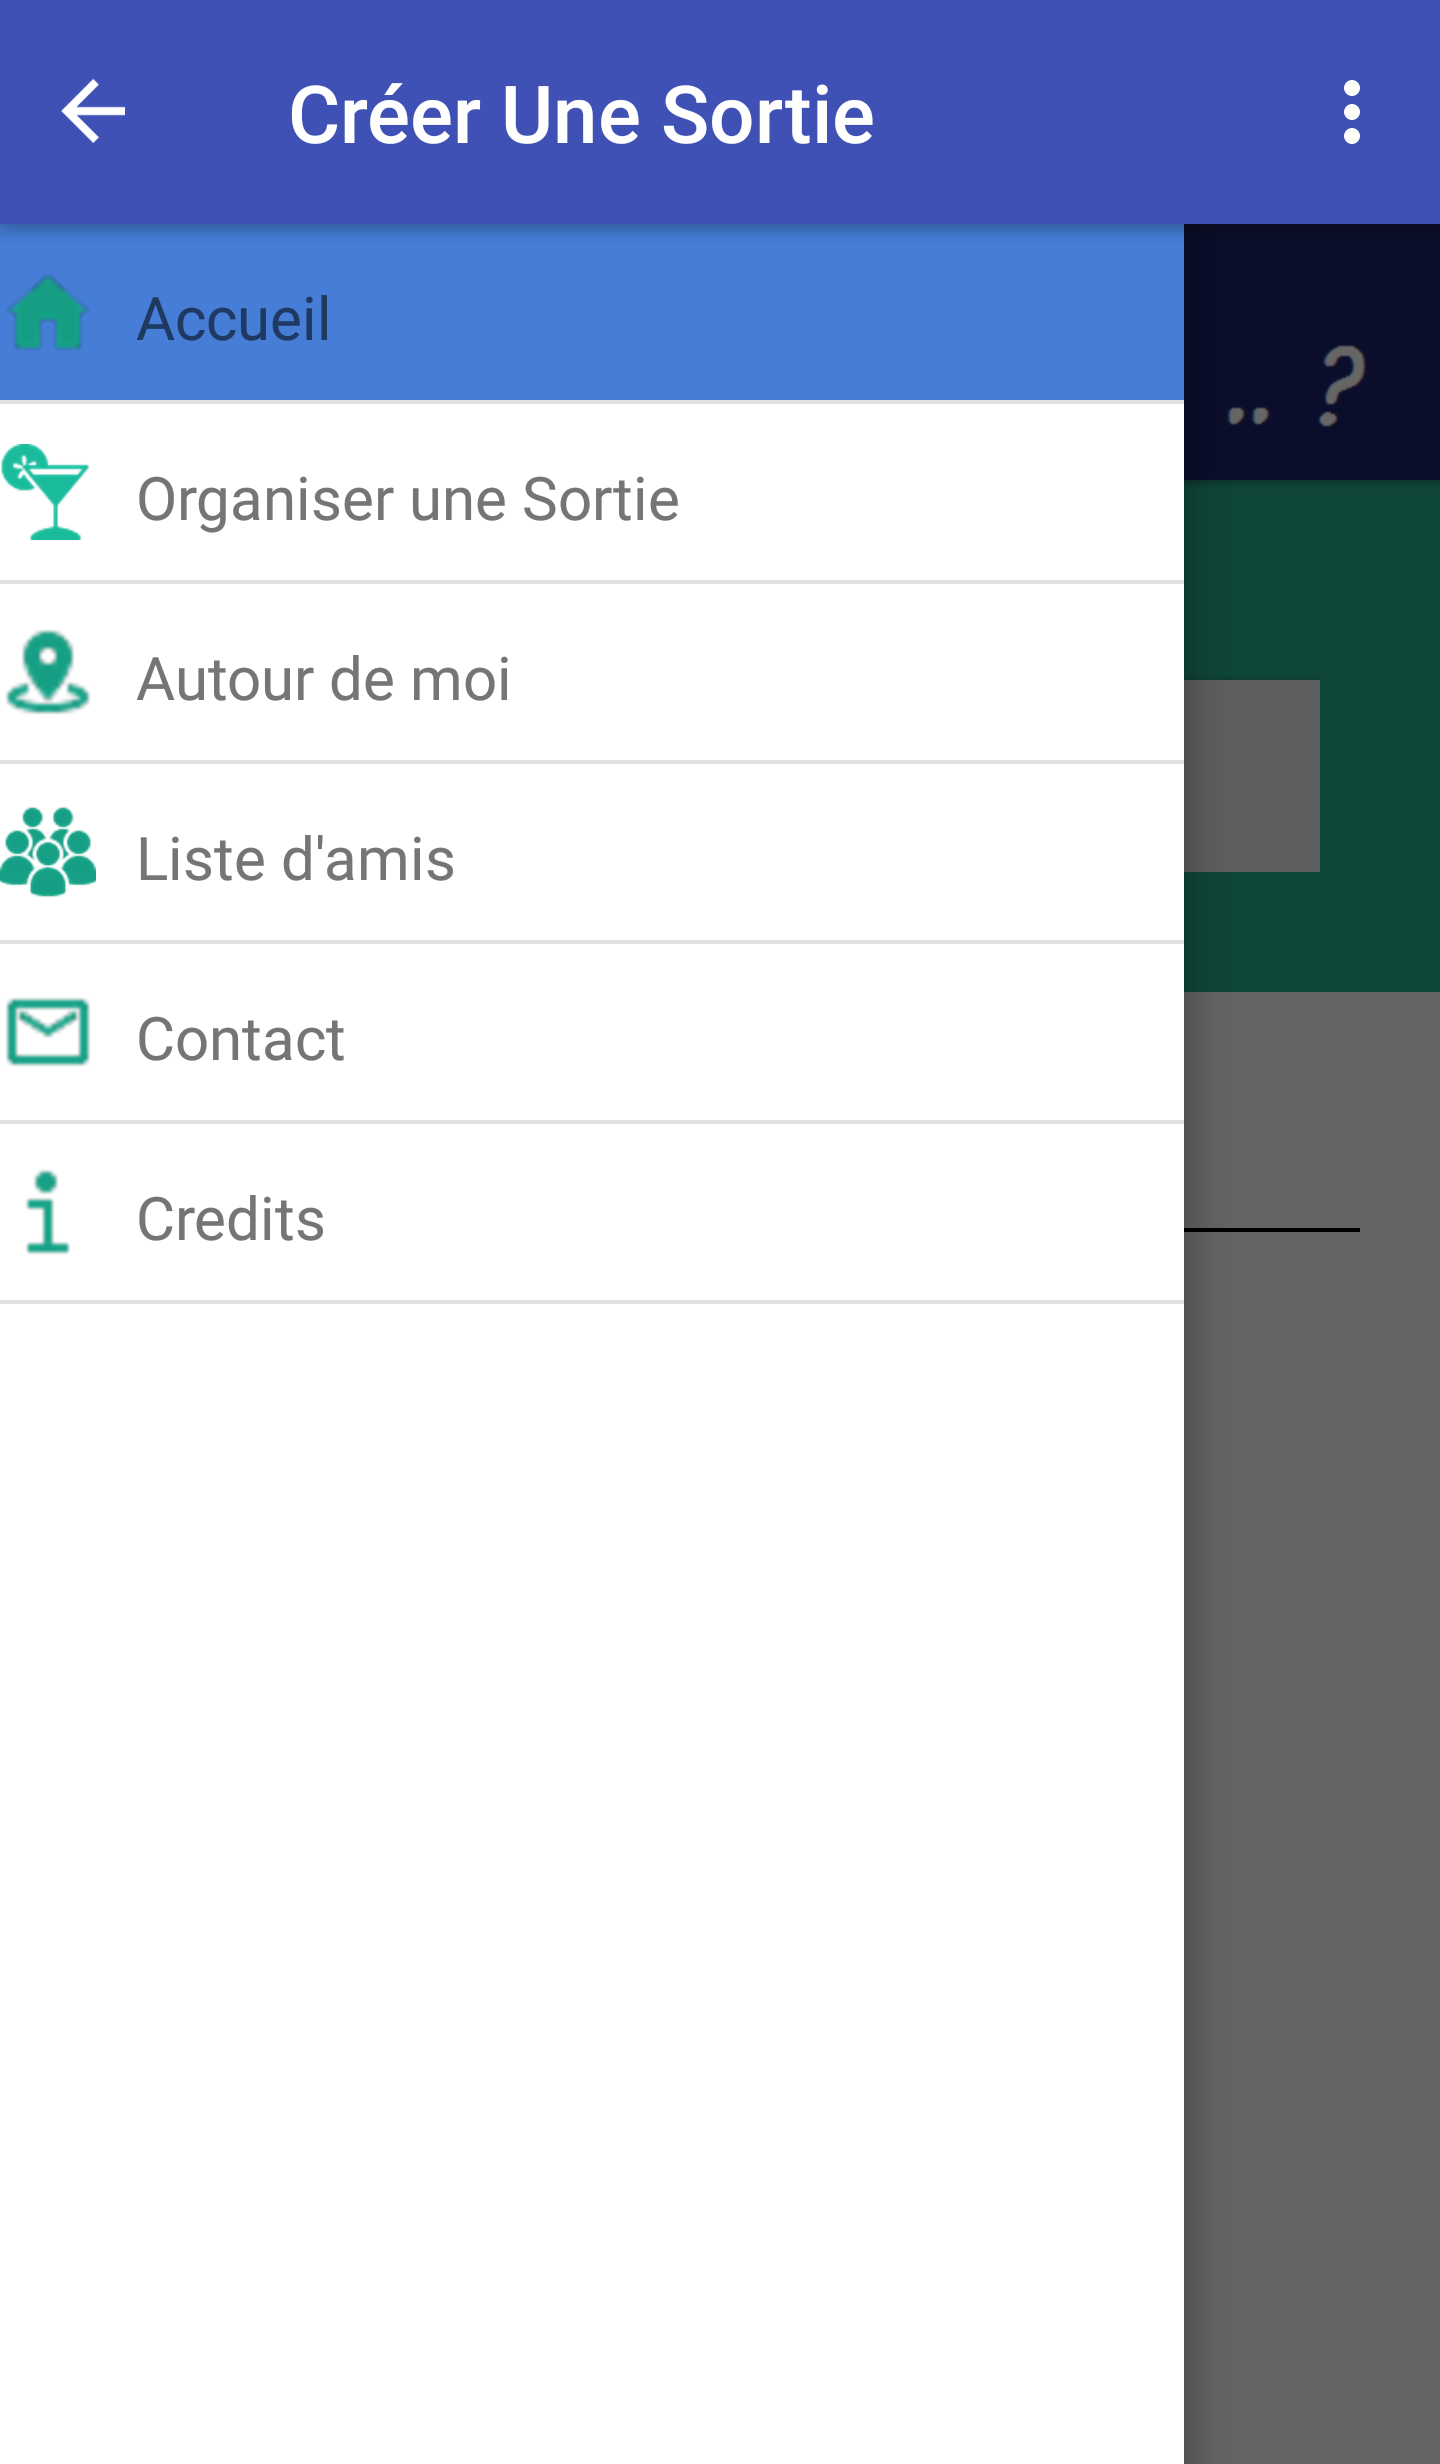
\includegraphics[height=0.4\textheight]{Interface_Menu.png}
    \label{interface:MenuAccueil}}
    \hfill
\end{figure}
\vfill

\begin{figure}[!htb]
    \centering
    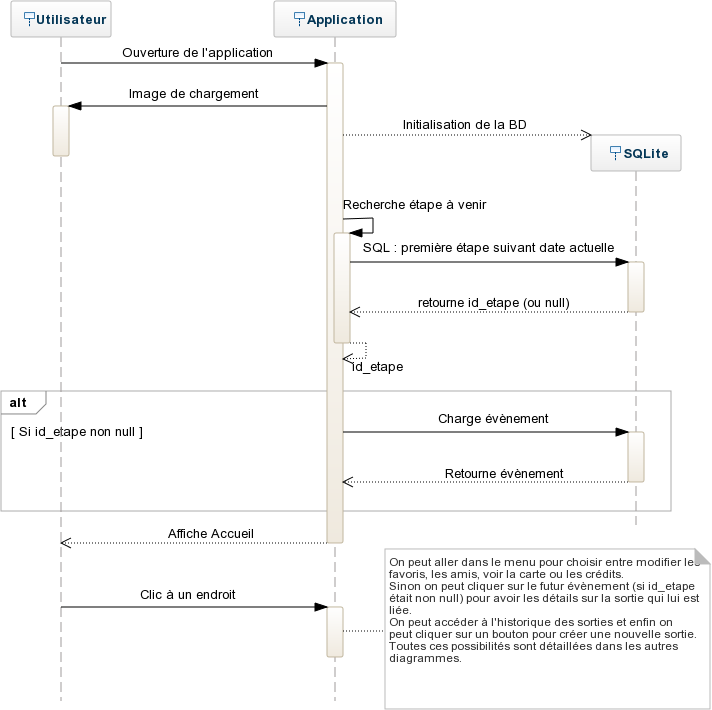
\includegraphics[width=1\textwidth]{Sequence_Accueil.png}
    \caption[Diagramme de séquence de l'accueil]{Diagramme de séquence représentant le déroulement interne de l'application lors de son démarrage}
    \label{fig:Accueil}
\end{figure}
\clearpage


\section{Création d'une sortie}
La création d'une sortie s'effectue en plusieurs étapes qui seront détaillées séparément dans les sections suivantes.

\subsection{Initialisation de la sortie}
Il est tout d’abord nécessaire d'initialiser la sortie; c'est à dire donner les informations de base qui permettront de la différencier des autres : un nom, un lieu, une date, un moyen de transport et des participants (ce dernier point sera traité dans la prochaine section).

L'interface est donc très simple (interface \ref{interface:CreerSortie}) tout comme son fonctionnement (diagramme \ref{fig:InitSortie}, ne demandant qu'à remplir les champs et cliquer sur son moyen de transport.

\vfill
\begin{figure}[!htb]
    \centering
    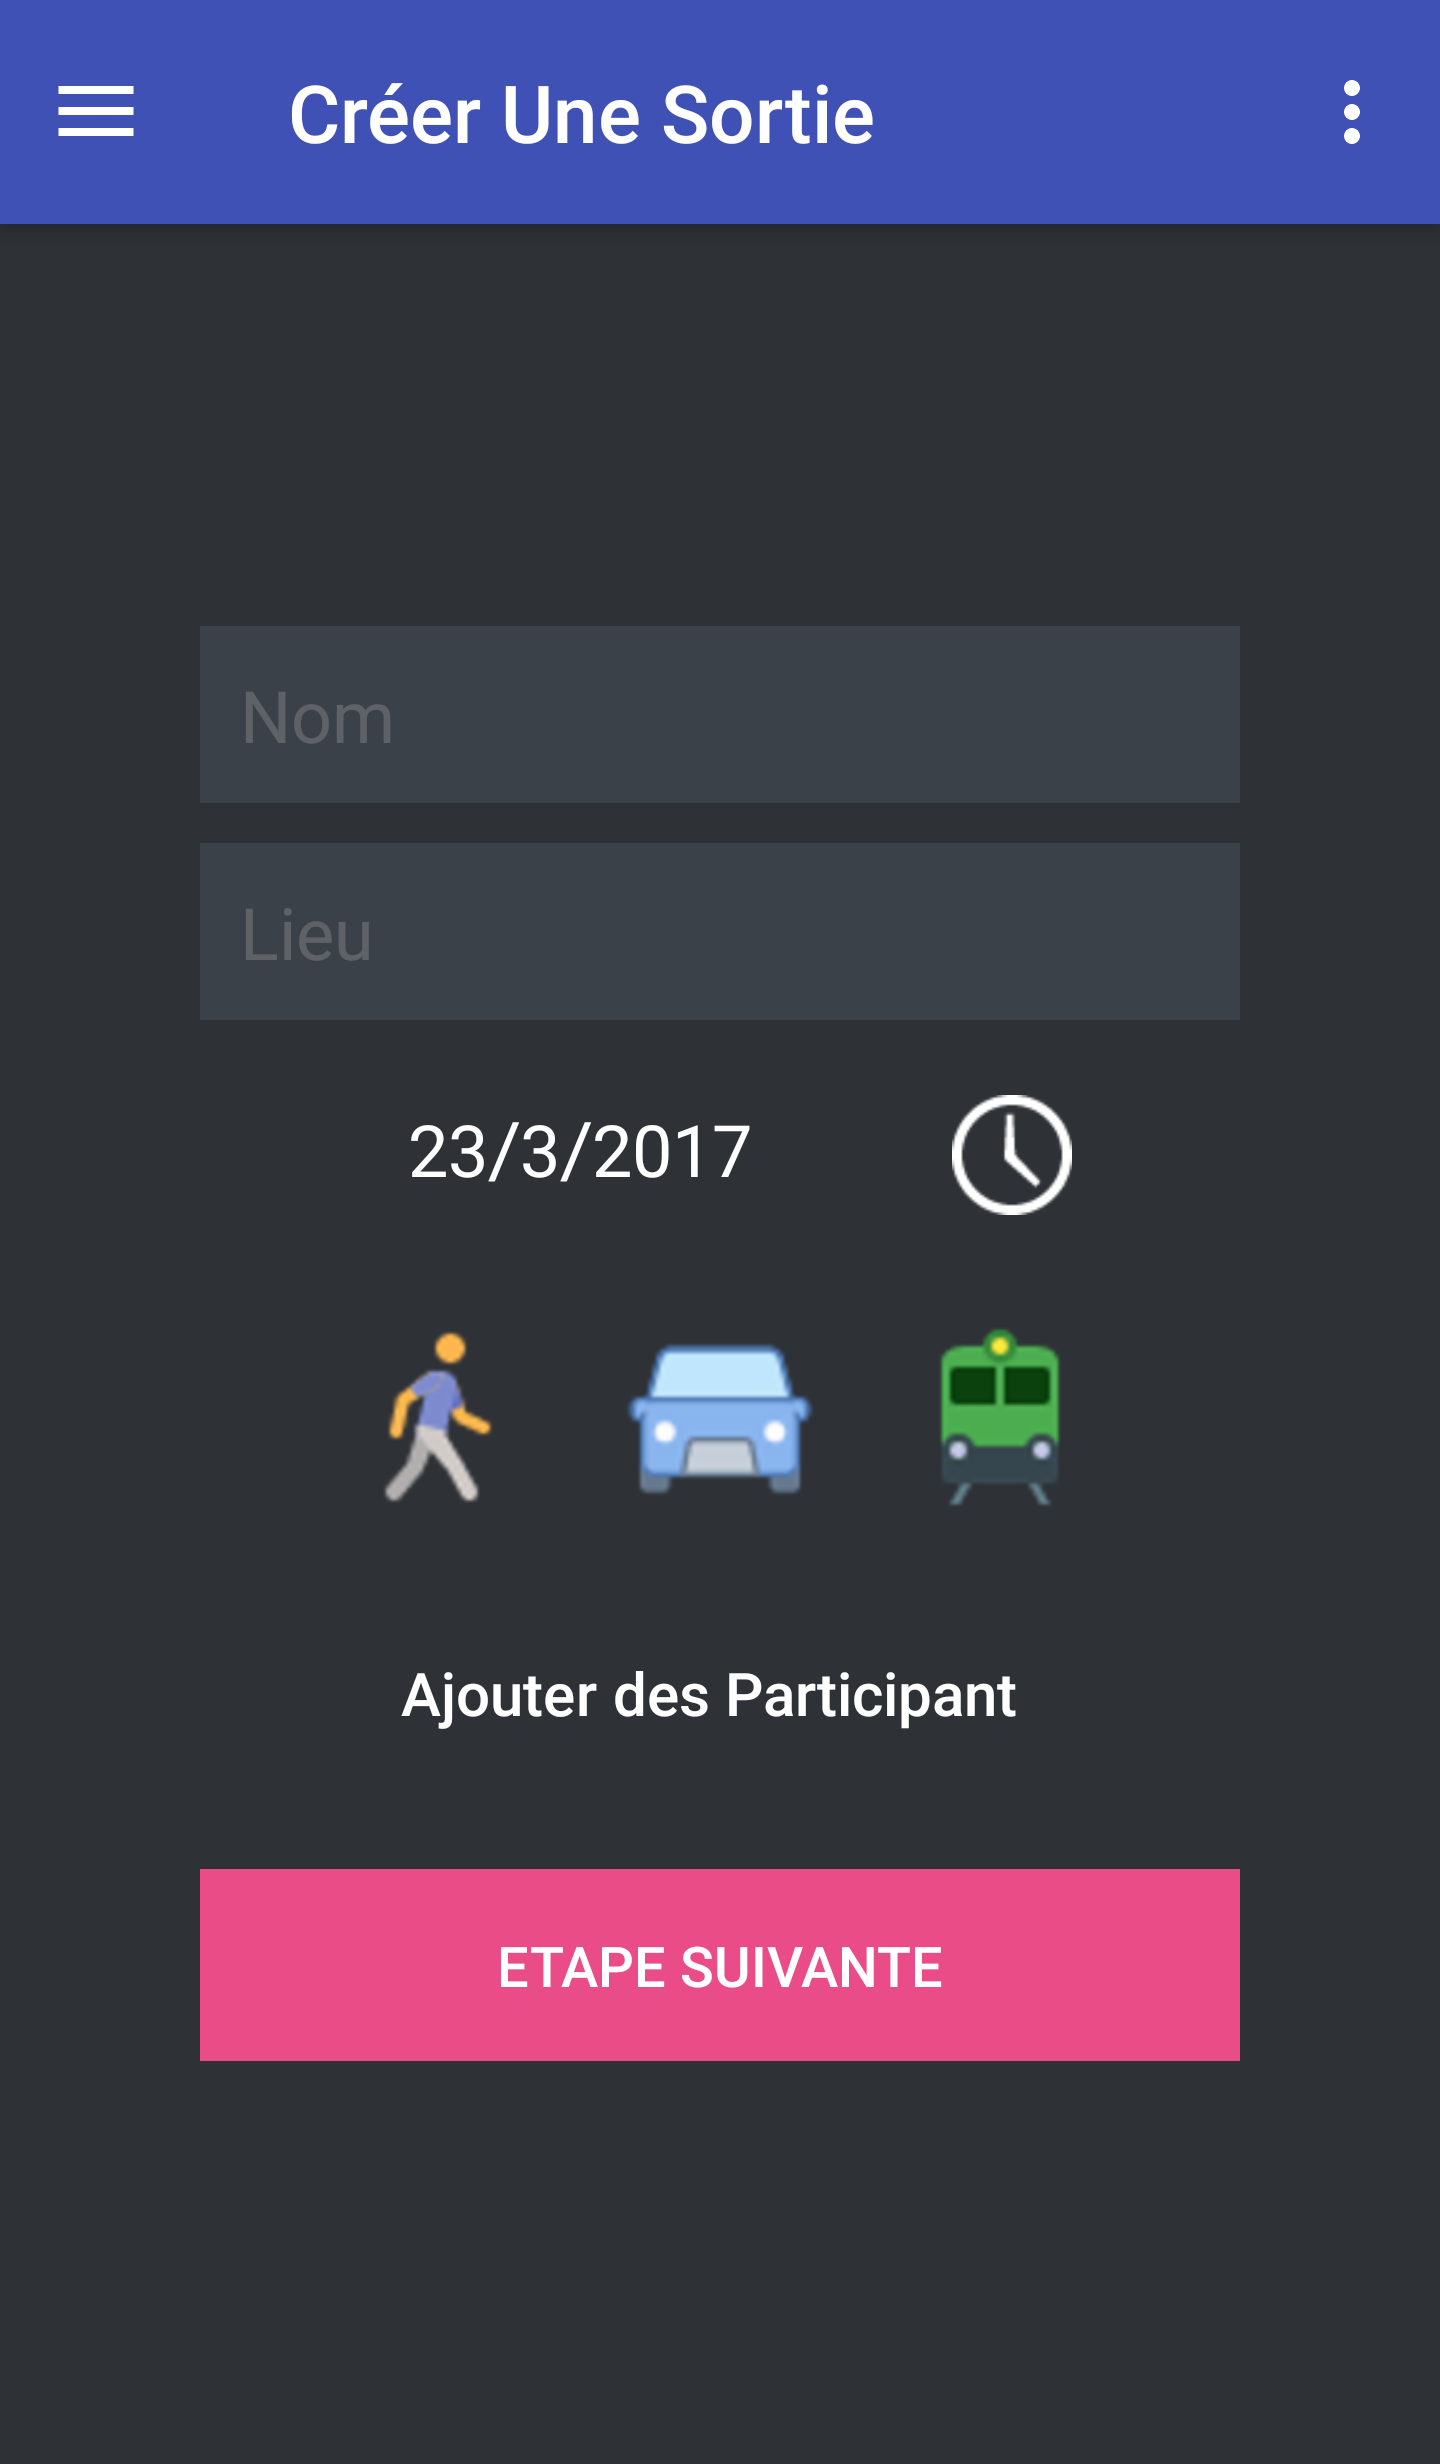
\includegraphics[height=0.4\textheight]{Interface_Creer_Sortie.png}
    \caption[]{Interface permettant d’initialiser une nouvelle sortie}
    \label{interface:CreerSortie}
\end{figure}
\vfill

\begin{figure}[!htb]
    \centering
    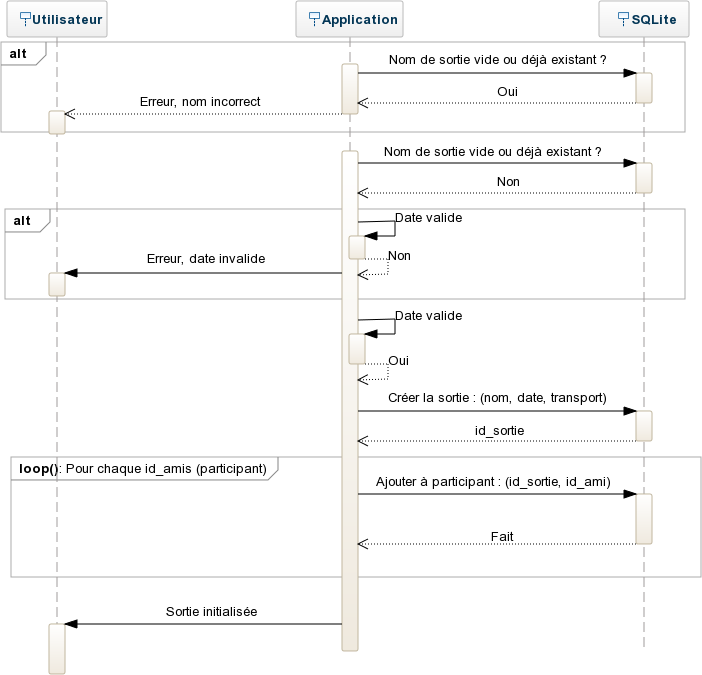
\includegraphics[width=1\textwidth]{Sequence_Initialisation_Sortie.png}
    \caption[Diagramme de séquence d'initialisation de sortie]{Diagramme de séquence représentant les étapes et les cas d'erreur lors de l'initialisation d'une nouvelle sortie}
    \label{fig:InitSortie}
\end{figure}
\clearpage

\subsection{Ajout de participants}
Chaque participant peut être ajouté de plusieurs manières différentes (interface \ref{interface:choixParticipant}) : soit en le sélectionnant depuis la liste des amis (d'anciens participants), soit en en créant un nouveau (interface \ref{interface:newParticipant}). Un participant peut alors être importé depuis sa liste de contacts et complété si besoins est.

Si l'utilisateur vient de créer un participant, il sera ajouté en plus à sa liste d'amis.

\vfill
\begin{figure}[!htb]
    \centering
    \subfloat[Choix entre créer un participant ou en sélectionner un ancien]
    {\label{interface:choixParticipant}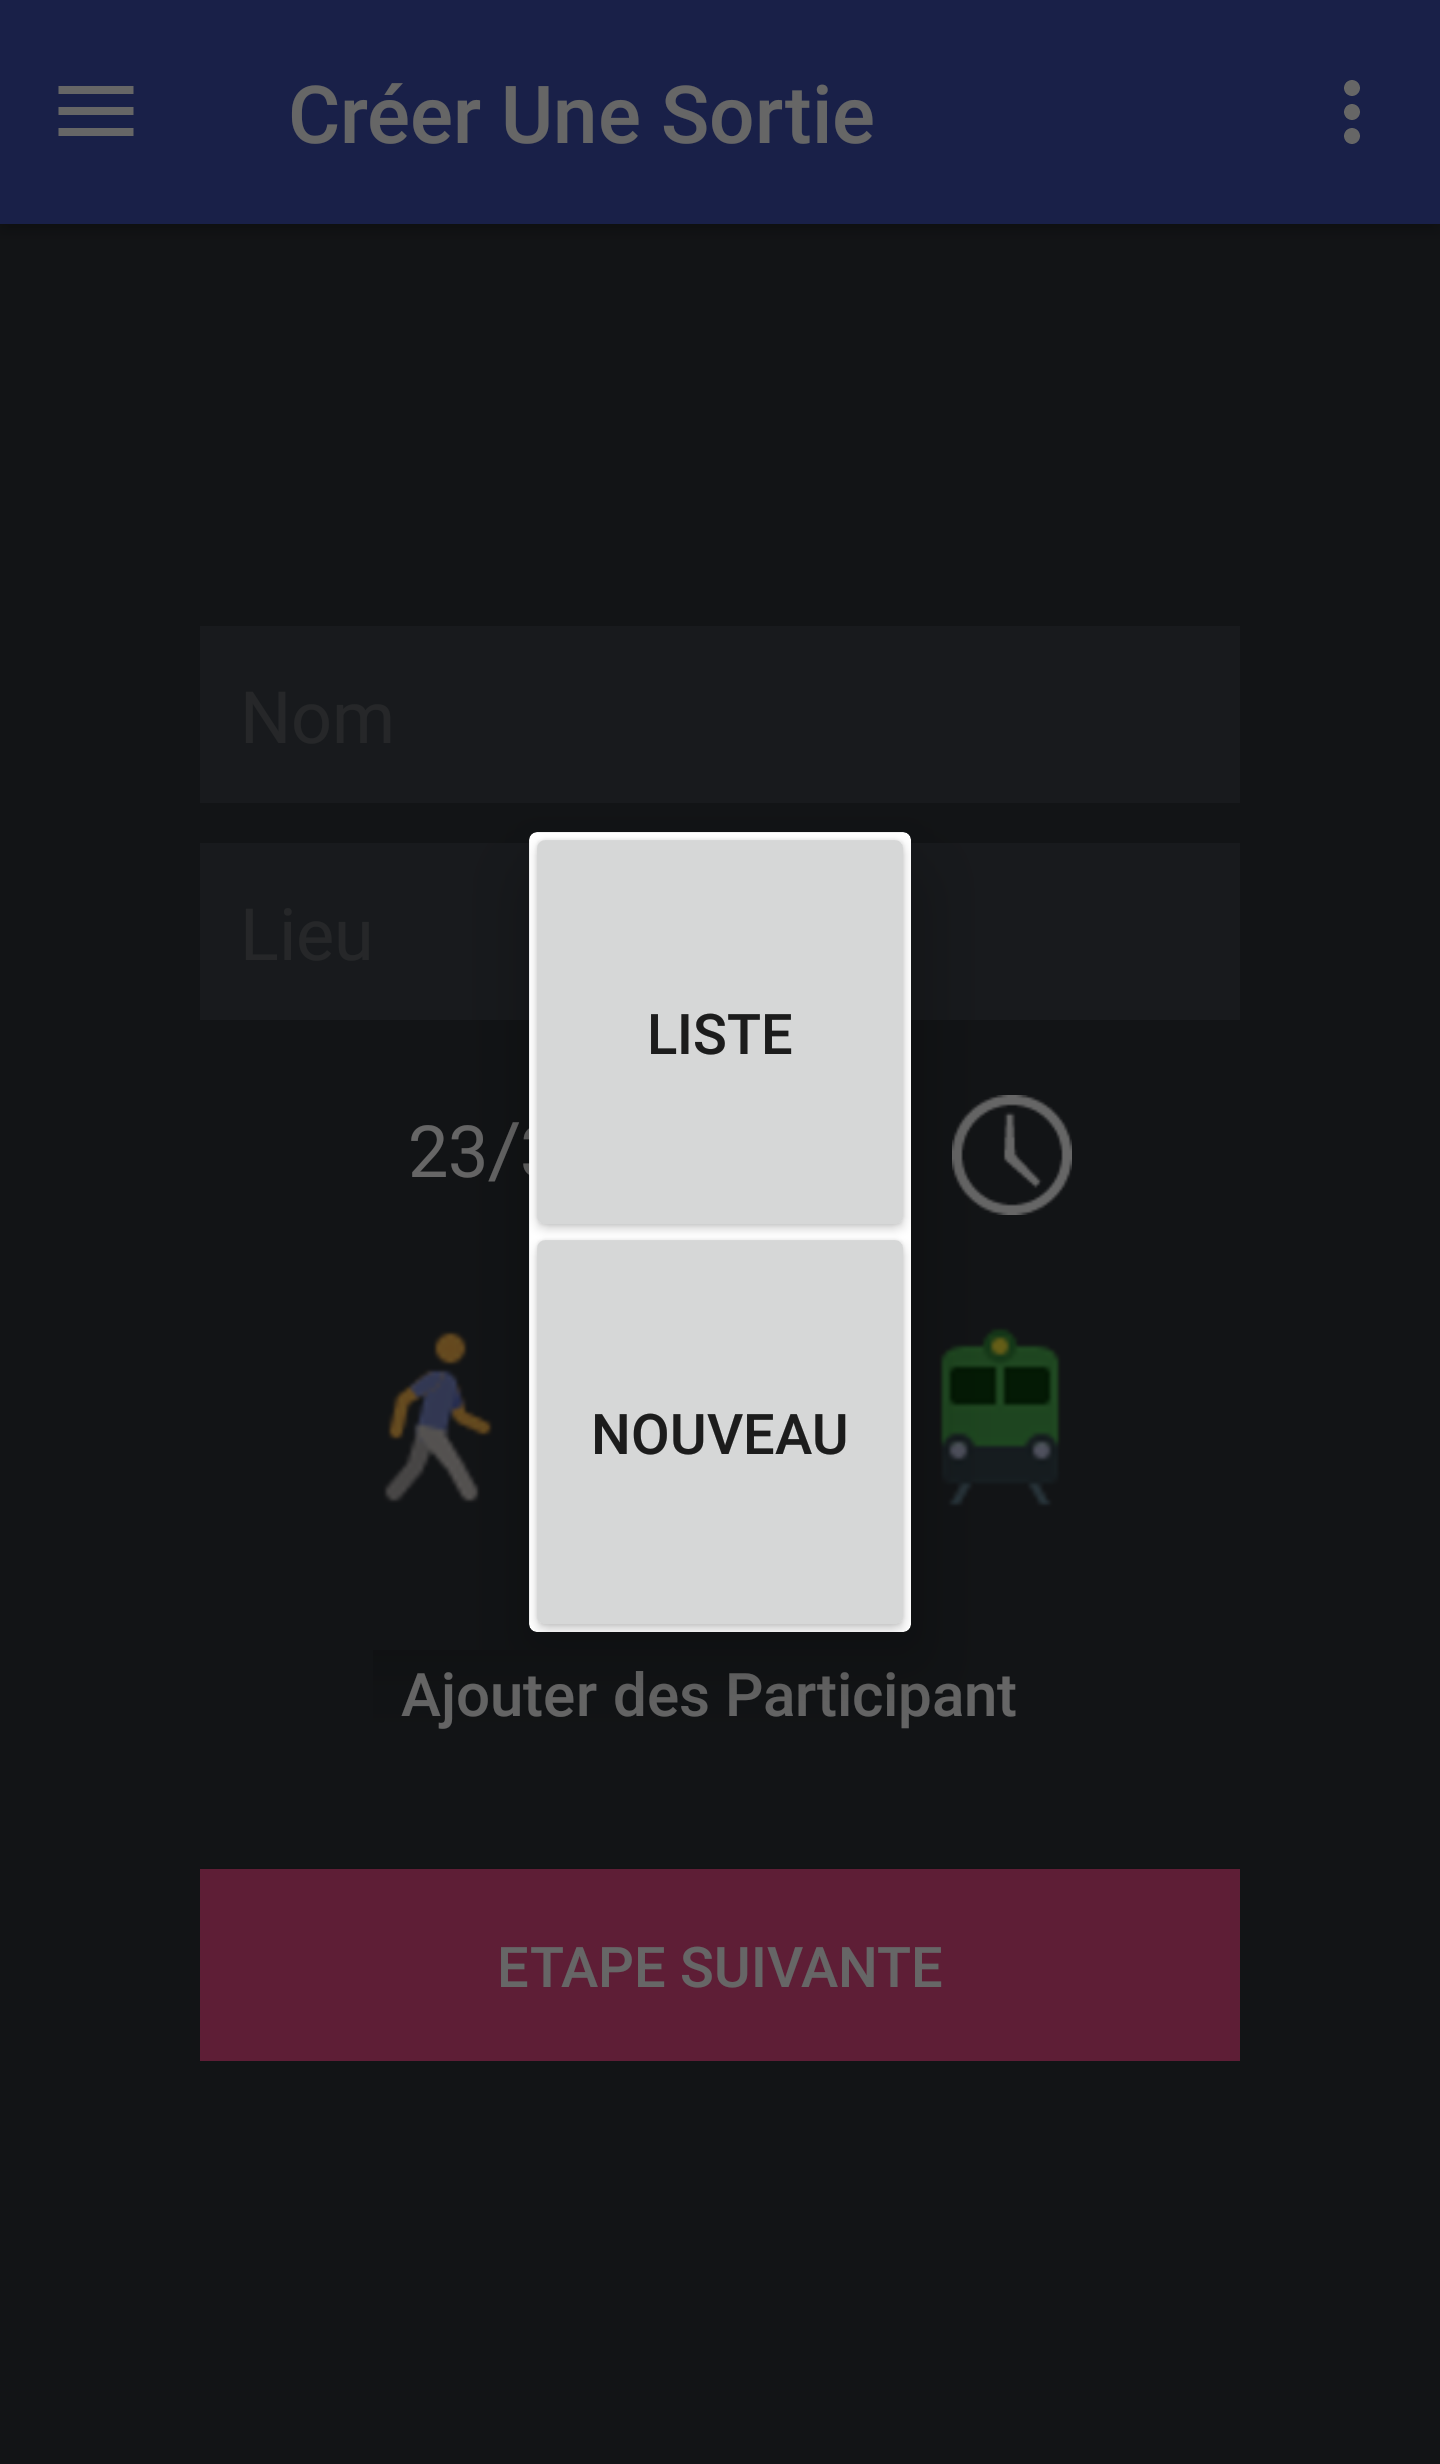
\includegraphics[height=0.4\textheight]{Interface_Choix_Ajout_Participant.png}}
    \hfil
    \subfloat[Création d'un nouveau participant]
    {\label{interface:newParticipant}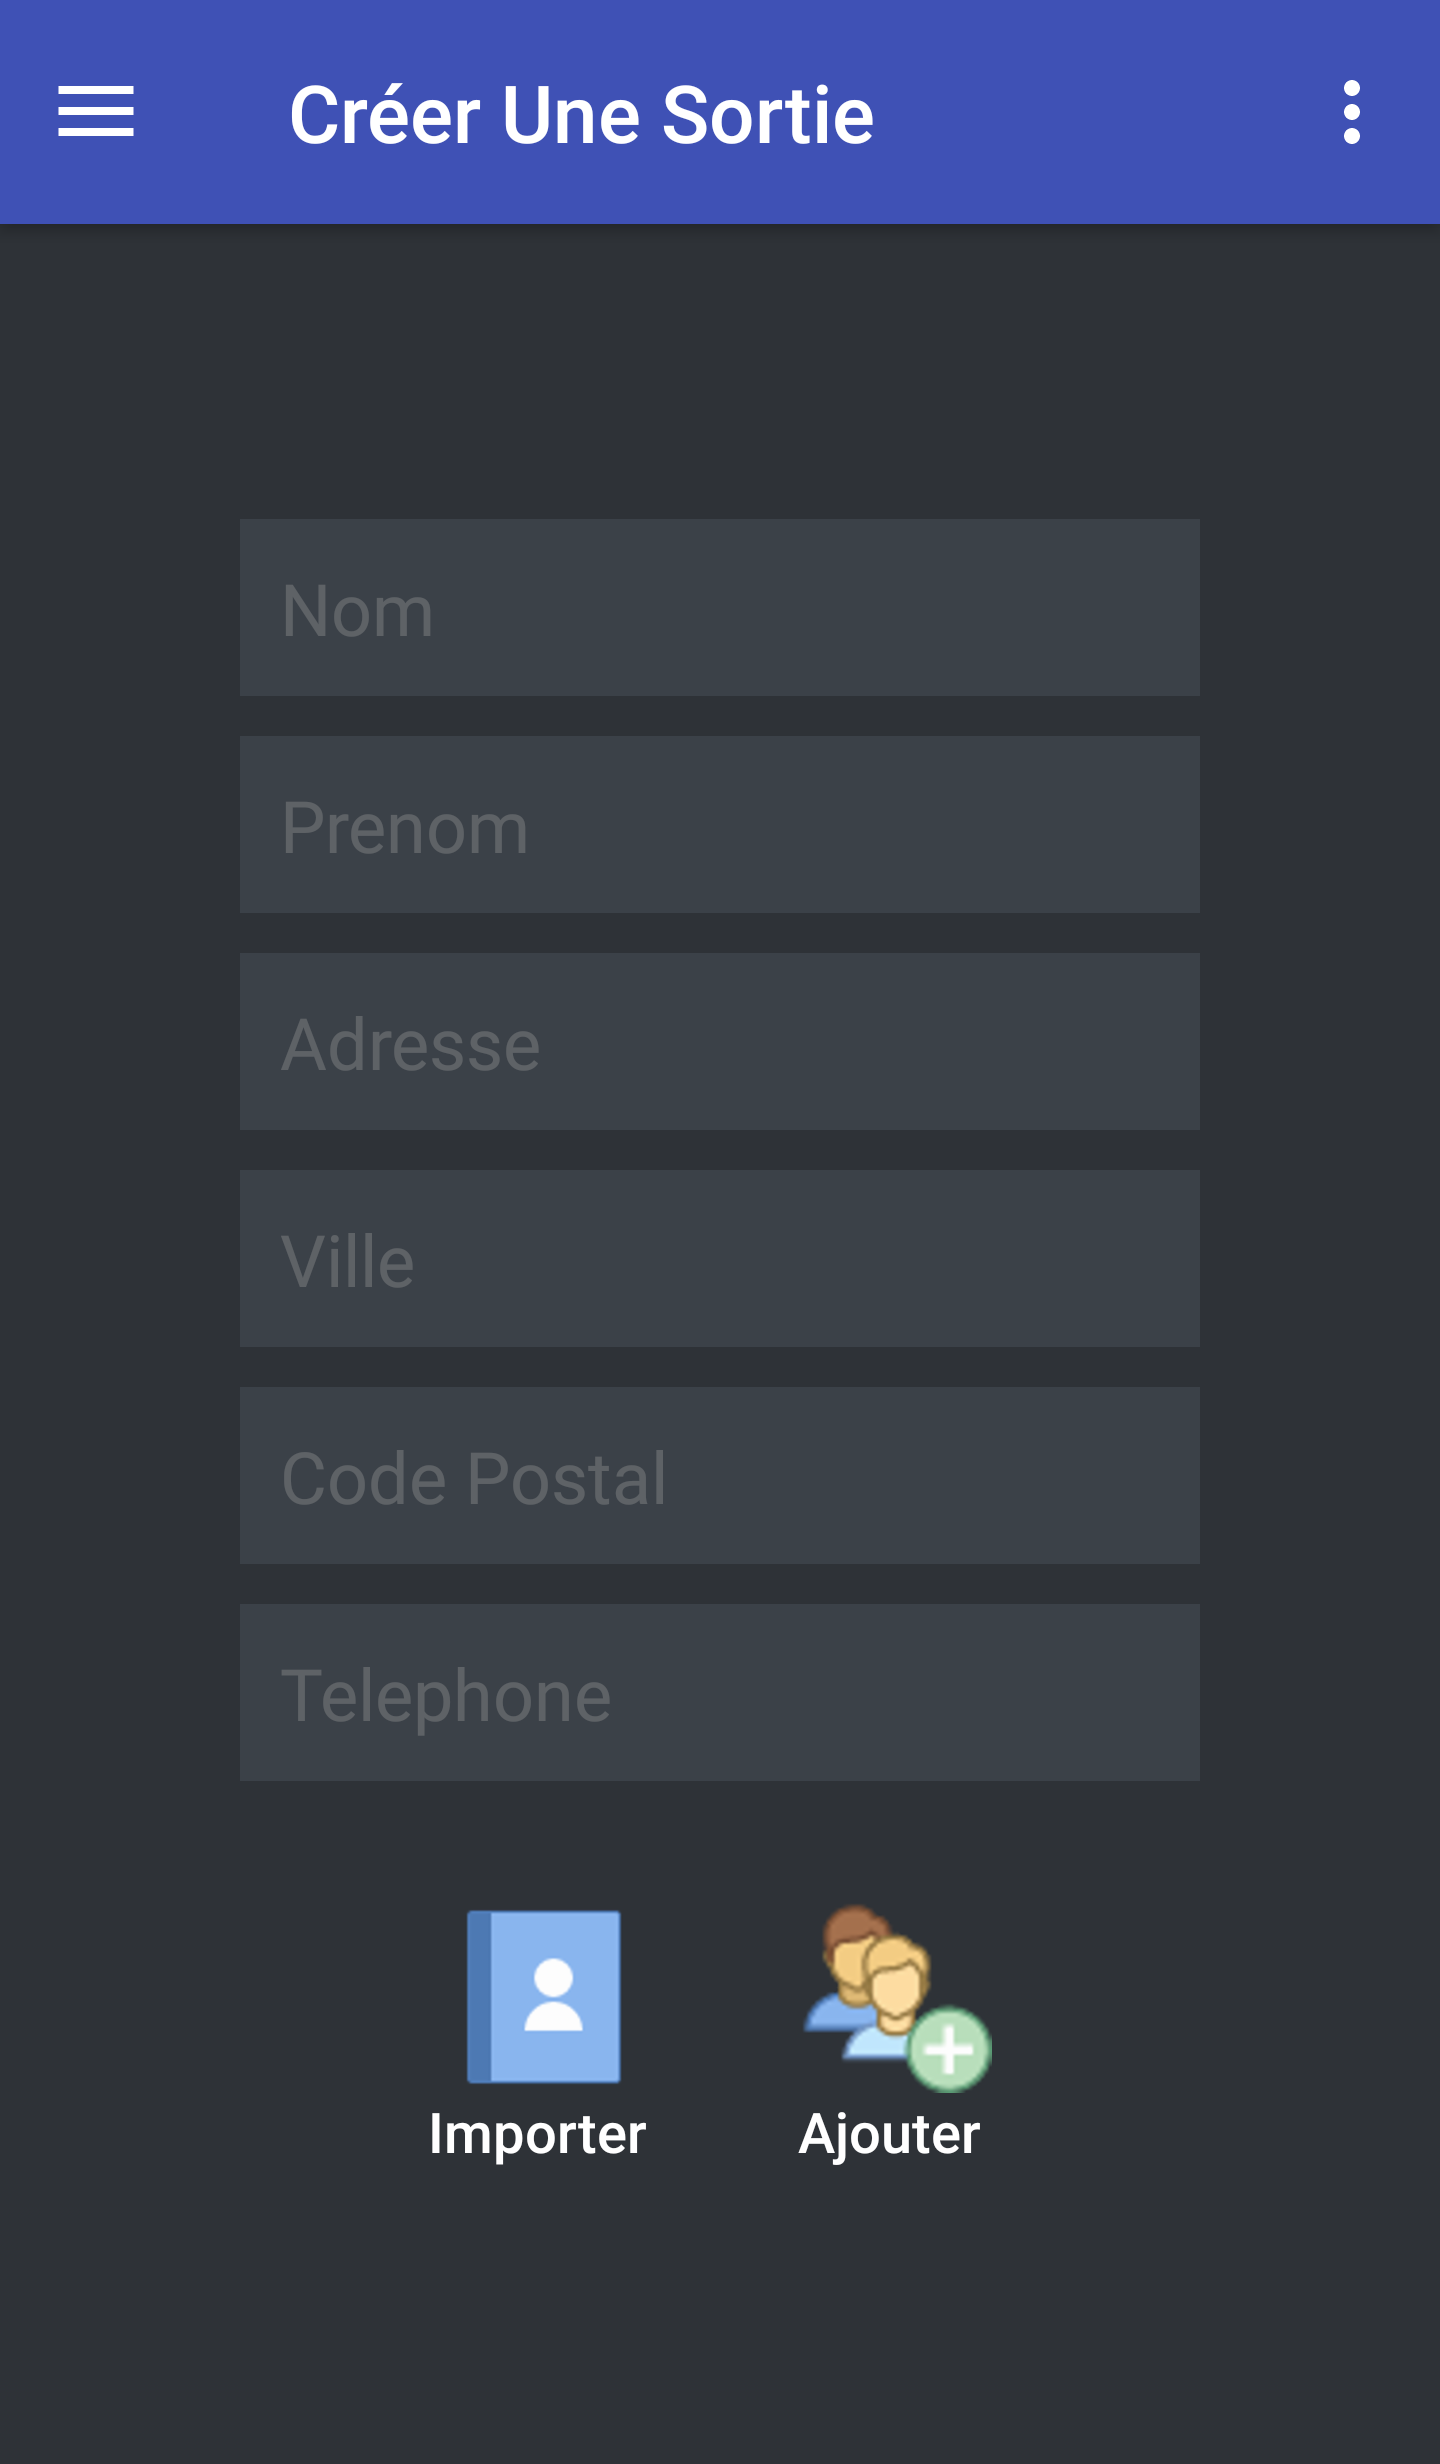
\includegraphics[height=0.4\textheight]{Interface_Ajout_Participant.png}}
    \caption[]{Interfaces permettant d'ajouter des participants à la sortie}
    \label{interface:AjoutParticipant}
\end{figure}
\vfill
\clearpage

\subsection{Choix des étapes}
Vient ensuite l'étape permettant de définir les étapes de la sortie ainsi que leur ordre.
Pour cela, l'interface \ref{interface:etapeBase} affichera les différents endroits possibles qu'il suffira de tapoter dans l'ordre voulu (exemple avec l'interface \ref{interface:ChangeEtapes}).
Pour supprimer une étape il suffit de tapoter à nouveau dessus.

Tout cela est détaillé dans le diagramme \ref{fig:ChangeEtapes}.
\vfill
\begin{figure}[!htb]
    \centering
    \subfloat[Choix des étapes (avant sélection)]
    {\label{interface:etapeBase}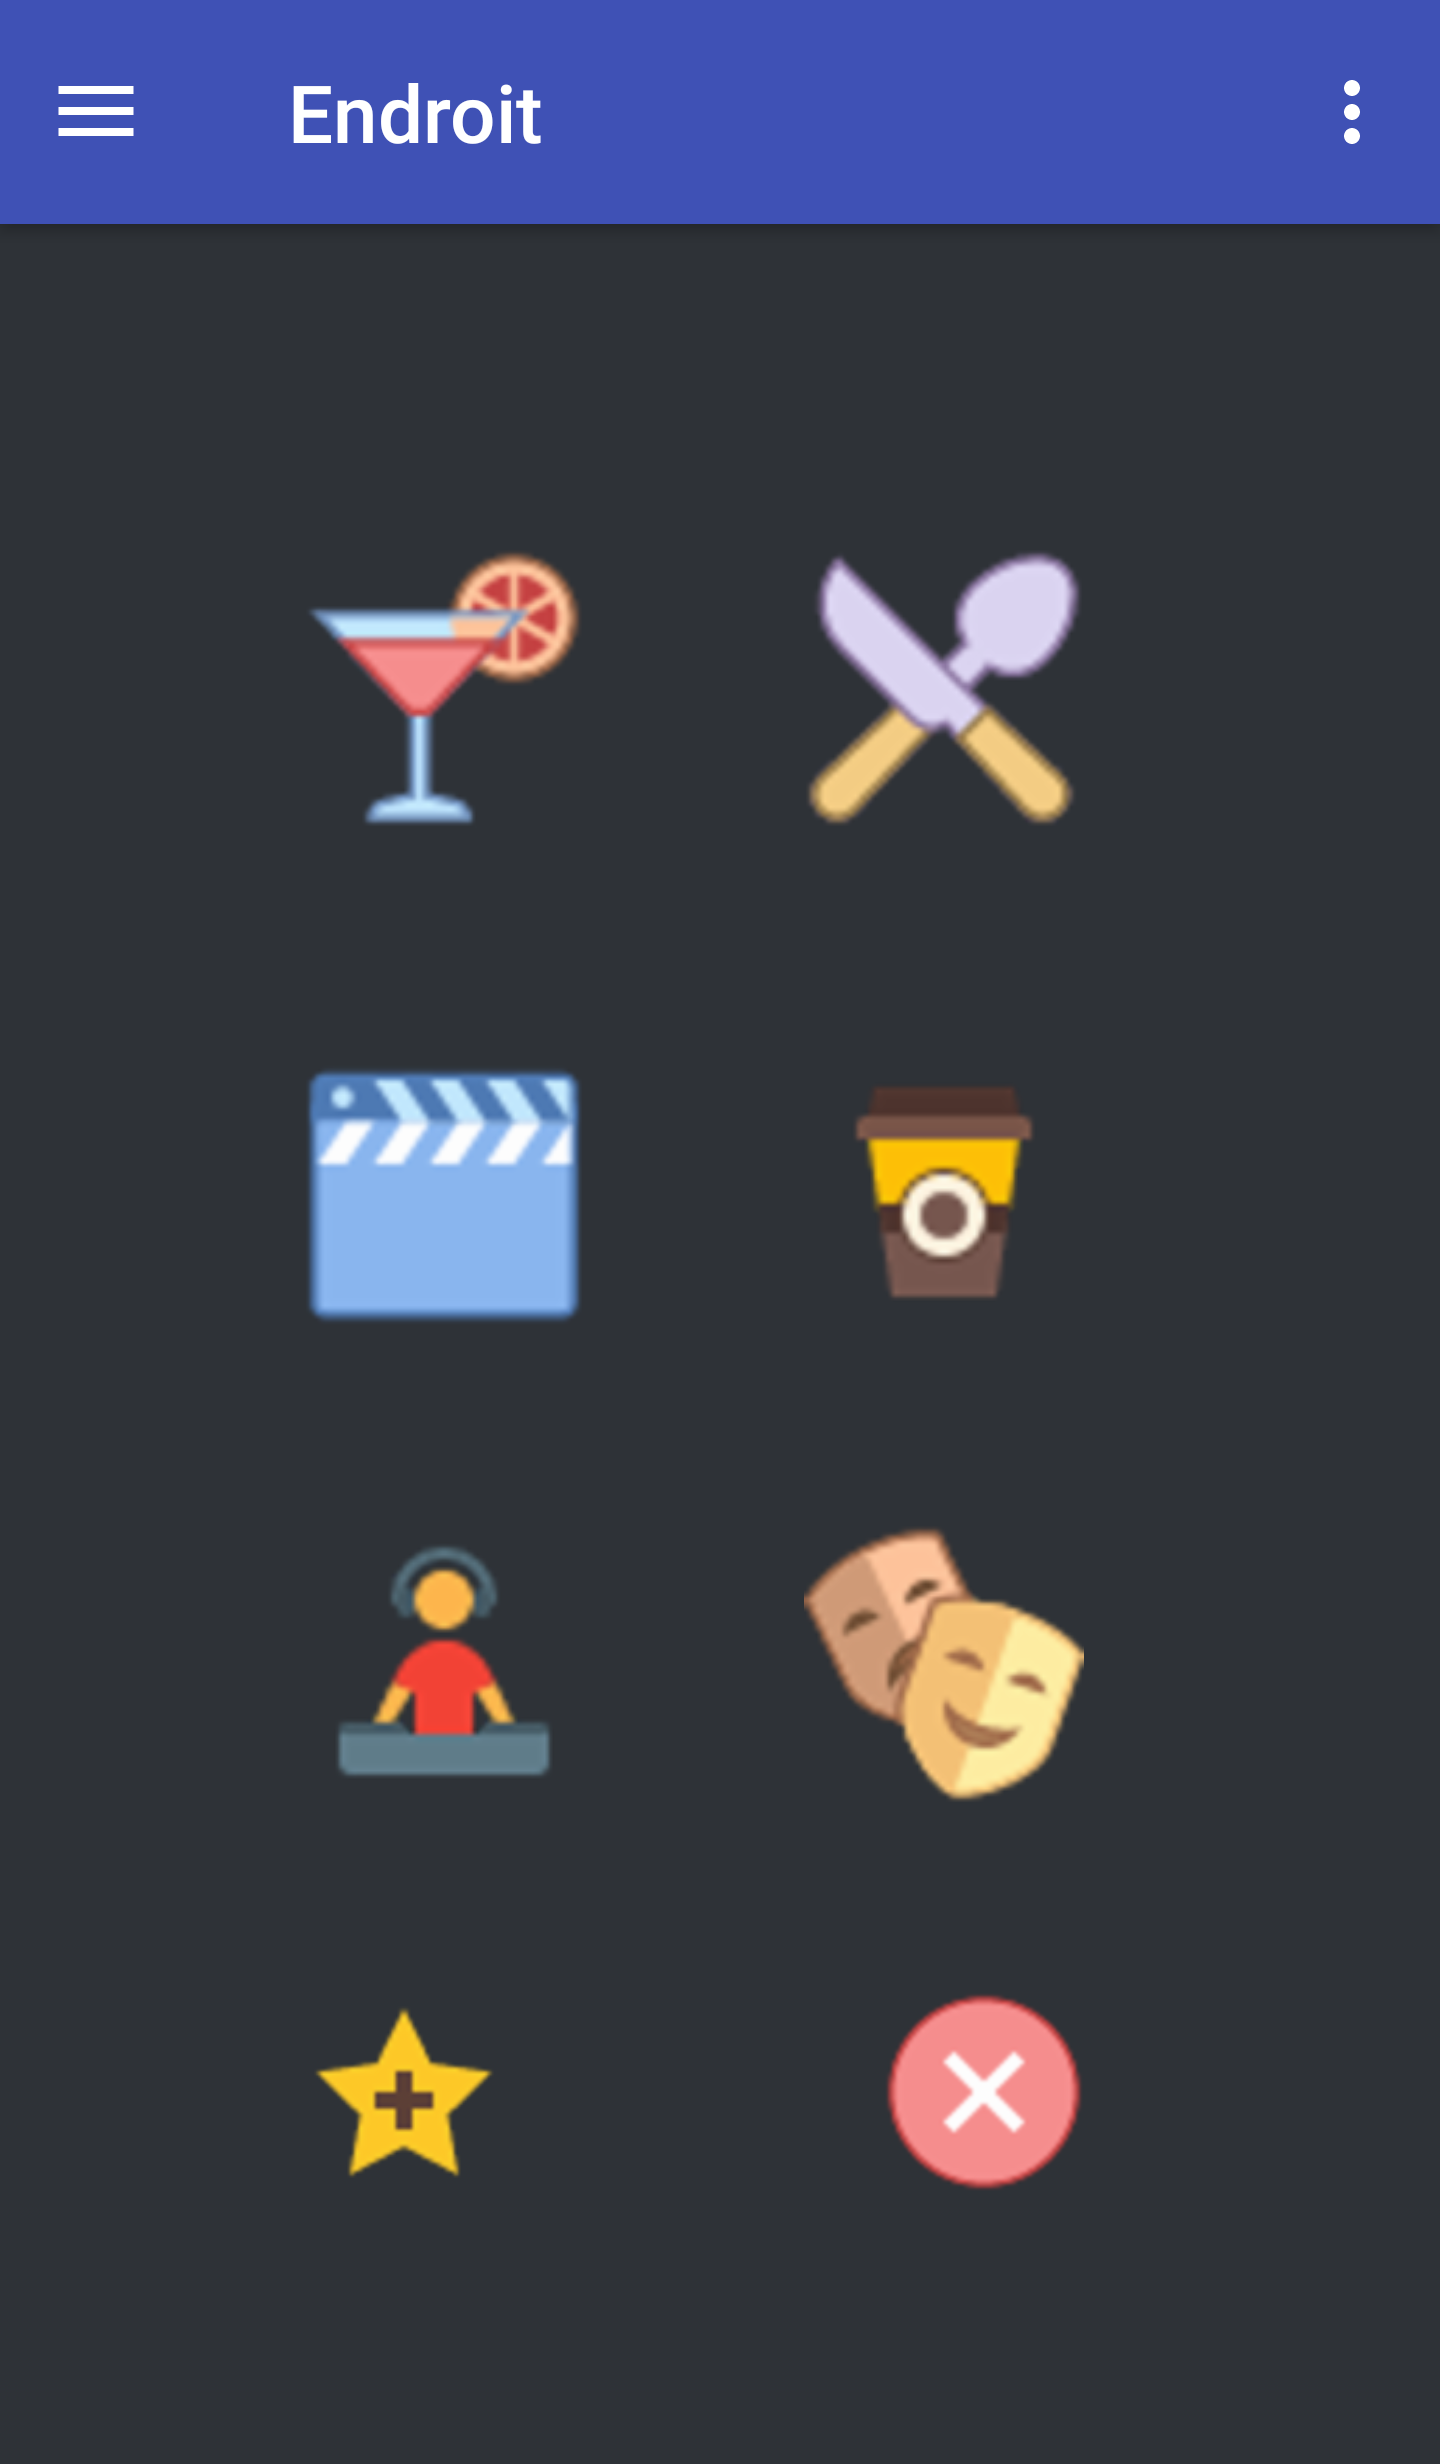
\includegraphics[height=0.4\textheight]{Interface_Etape_Base.png}}
    \hfil
    \subfloat[Choix des étapes (après en avoir sélectionné 3)]
    {\label{interface:etapeSelect}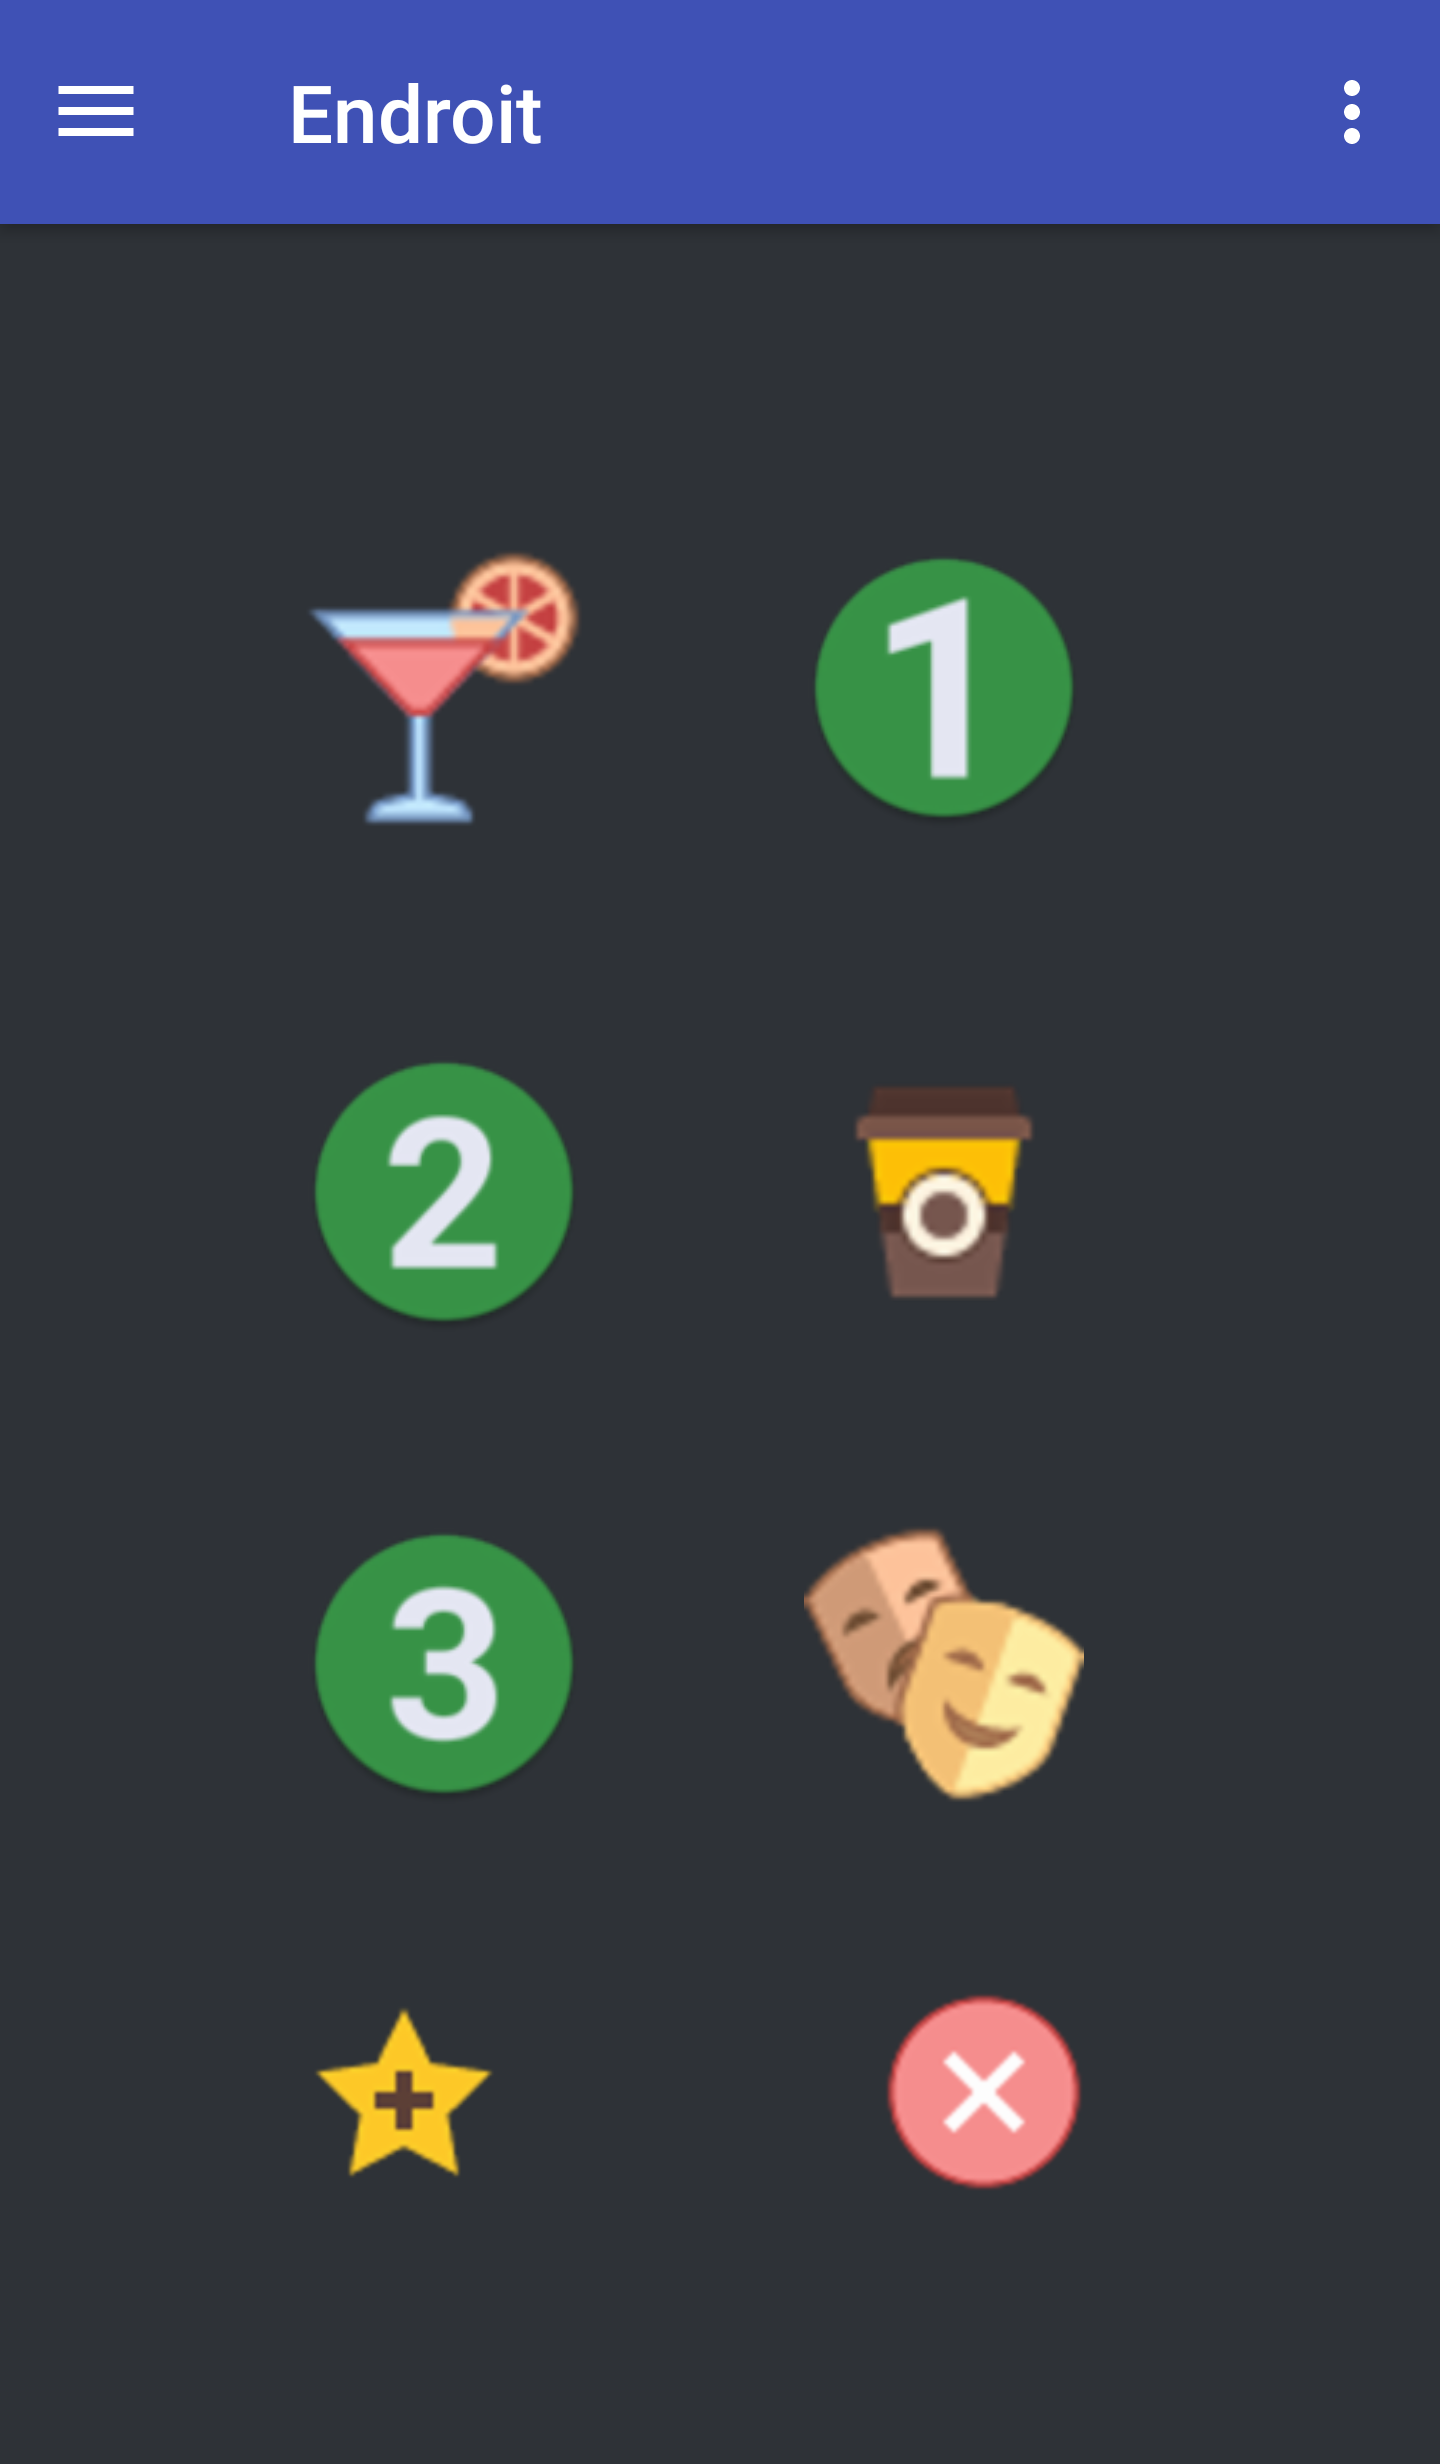
\includegraphics[height=0.4\textheight]{Interface_Etape_Selection.png}}
    \caption[]{Interfaces représentant le menu de choix des étapes, avant et après en avoir sélectionné}
    \label{interface:ChangeEtapes}
\end{figure}
\vfill

\begin{figure}[!htb]
    \centering
    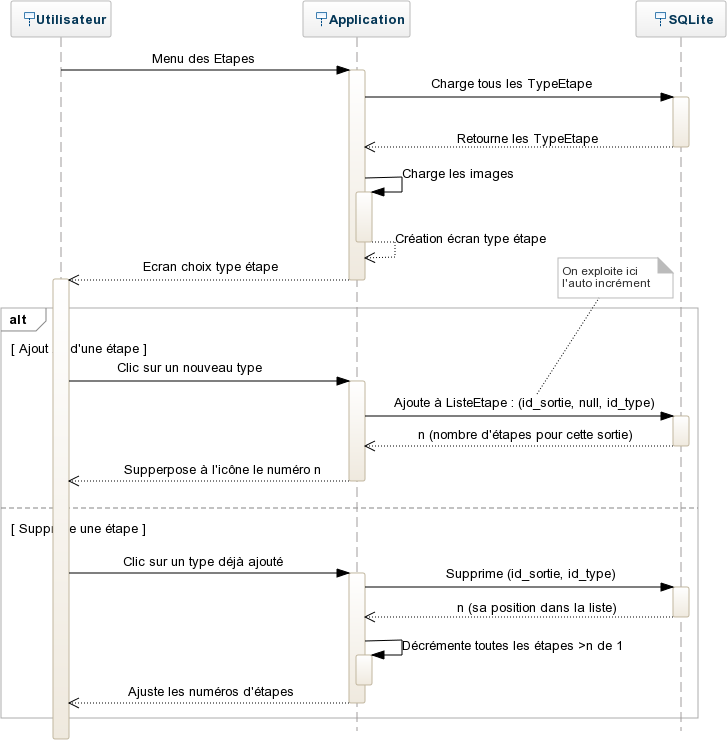
\includegraphics[width=1\textwidth]{Sequence_creer_une_liste_d_etapes.png}
    \caption[Diagramme de séquence de modification des étapes]{Diagramme de séquence représentant comment ajouter ou enlever une étape à la sortie}
    \label{fig:ChangeEtapes}
\end{figure}
\clearpage

\subsection{Choix des contraintes}
Les contraintes seront choisies parmi une liste de possibilités prédéfinies. Il sera possible d'en sélectionner autant que l'on veut.

\subsection{Calcul de la sortie idéale}
Le calcul de la sortie passant par la récupération d'adresses grâce à l'API de Google, une connexion internet sera obligatoire dans cette partie du programme.

L’algorithme utilisé est représenté par le diagramme \ref{fig:CalculSortie} et consiste simplement en un algorithme de parcours en largeur d'un arbre.
Cet arbre sera représenté à l'aide des classes \ref{fig:ClasseGraphe}, et sera construit ligne par ligne, en prenant bien en compte l'heure qu'il sera une fois arrivé à cette étape, l'heure qu'il sera une fois cette étape terminée, ainsi que toutes les contraintes que l'utilisateur aura éventuellement spécifié.

\vfill
\begin{figure}[!htb]
    \centering
    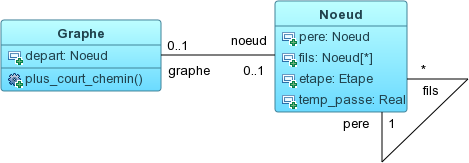
\includegraphics[width=0.5\textwidth]{Diagramme_de_classe_graphe.png}
    \caption[Diagramme de classe du graphe]{Diagramme de classe utilisé pour représenter un graphe orienté d'étapes}
    \label{fig:ClasseGraphe}
\end{figure}
\vfill
\vfill

\begin{figure}[!htb]
    \centering
    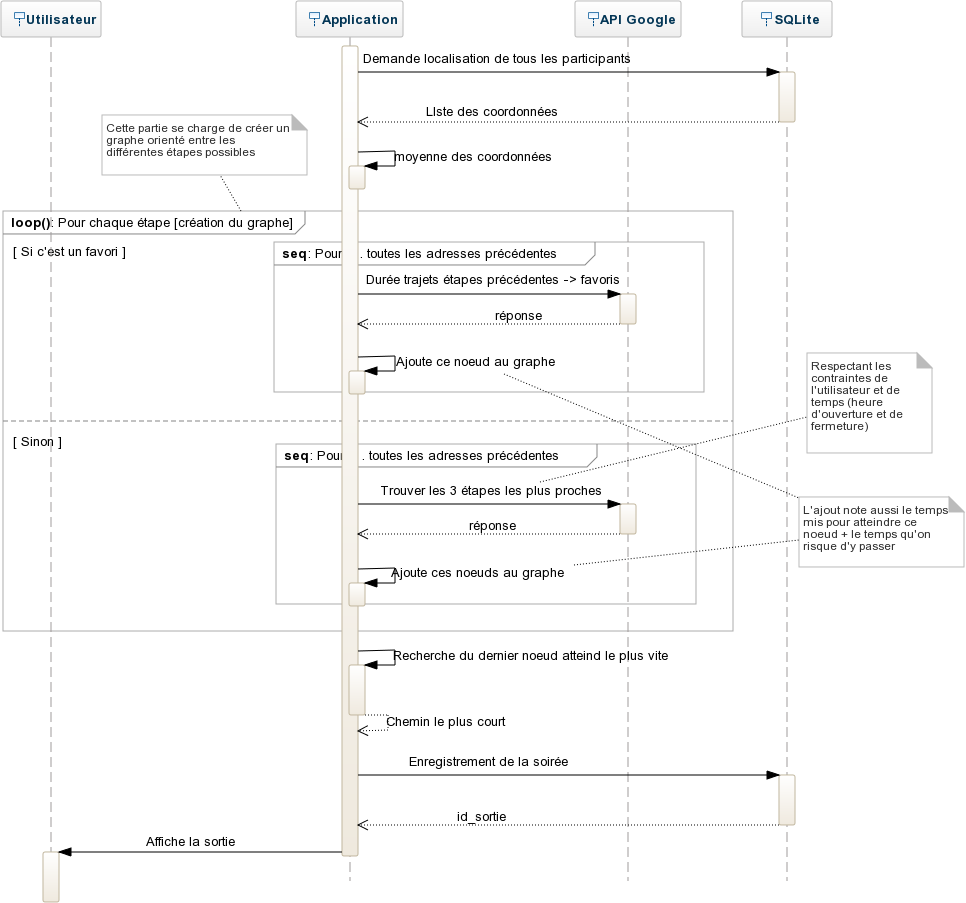
\includegraphics[width=1\textwidth]{Sequence_Calcul_Sortie.png}
    \caption[Diagramme de séquence de calcul de la sortie]{Diagramme de séquence représentant comment est calculé la sortie finale en fonction de tous les paramètres donnés précédemment}
    \label{fig:CalculSortie}
\end{figure}
\clearpage

\section{Favoris}
Le diagramme \ref{fig:Favoris} décrit comment l'utilisateur procède pour ajouter une adresse à sa liste des favoris. Cela peut se faire en cherchant un lieu sur la carte ou par le biais d'un formulaire.

\vfill
\begin{figure}[!htb]
    \centering
    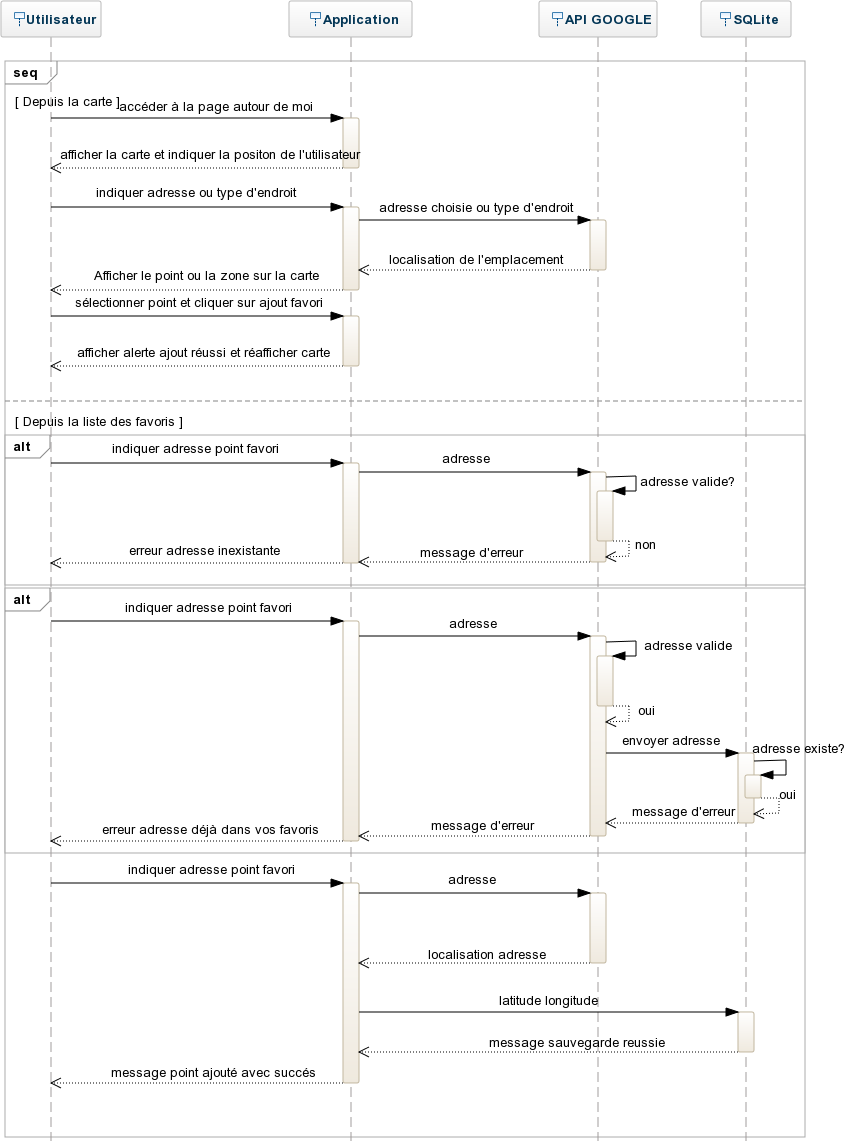
\includegraphics[width=0.9\textwidth]{Sequence_Favoris.png}
    \caption[Diagramme de séquence d'utilisation des favoris]{Diagramme de séquence représentant comment modifier ses favoris (que ce soit l'ajout ou la suppression)}
    \label{fig:Favoris}
\end{figure}
\vfill
\clearpage

\section{Carte}
La carte demandera elle aussi une connexion internet pour fonctionner correctement et exploitera une autre API de Google.
Une barre de recherche sera présente ainsi que la possibilité de tapoter à un endroit de la carte pour l'ajouter aux favoris (comme spécifier ci-dessous).  

\vfill
\begin{figure}[!htb]
    \centering
    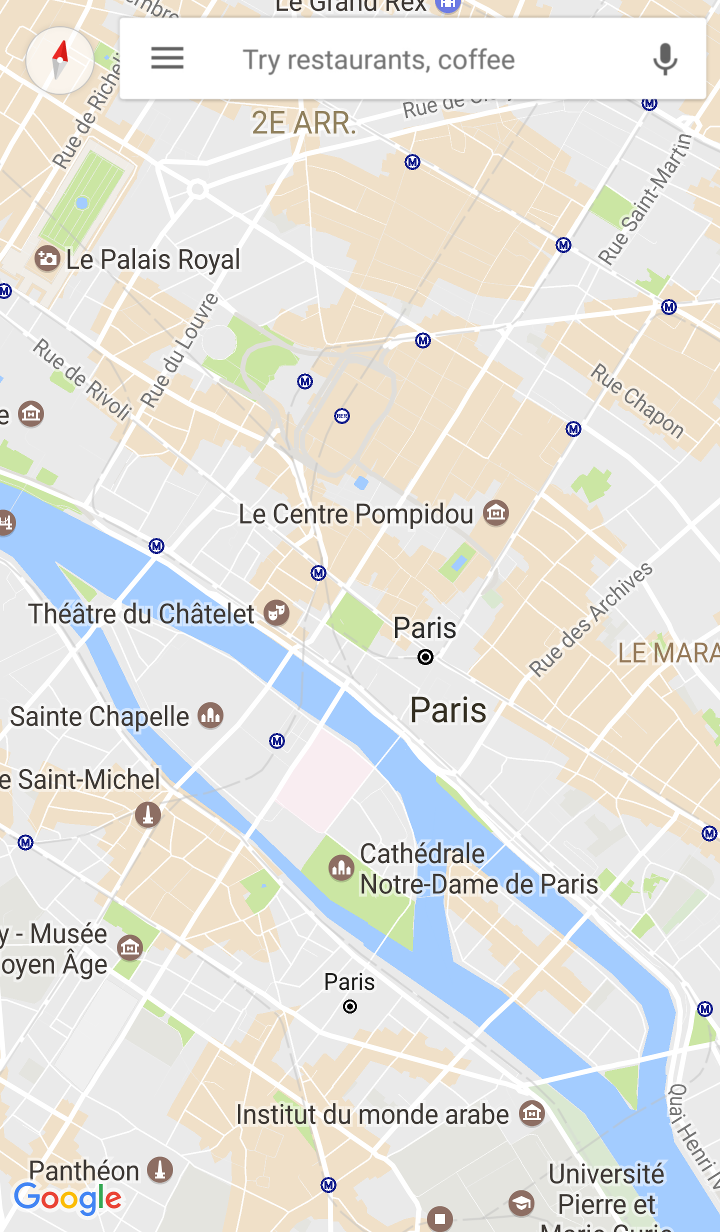
\includegraphics[height=0.4\textheight]{Interface_Carte.png}
    \caption[]{Interfaces représentant la carte}
    \label{interface:carte}
\end{figure}
\vfill
\vfill
\clearpage

\section{Tests}
\subsection{Tests unitaires}
\begin{figure}[!htb]
    \centering
    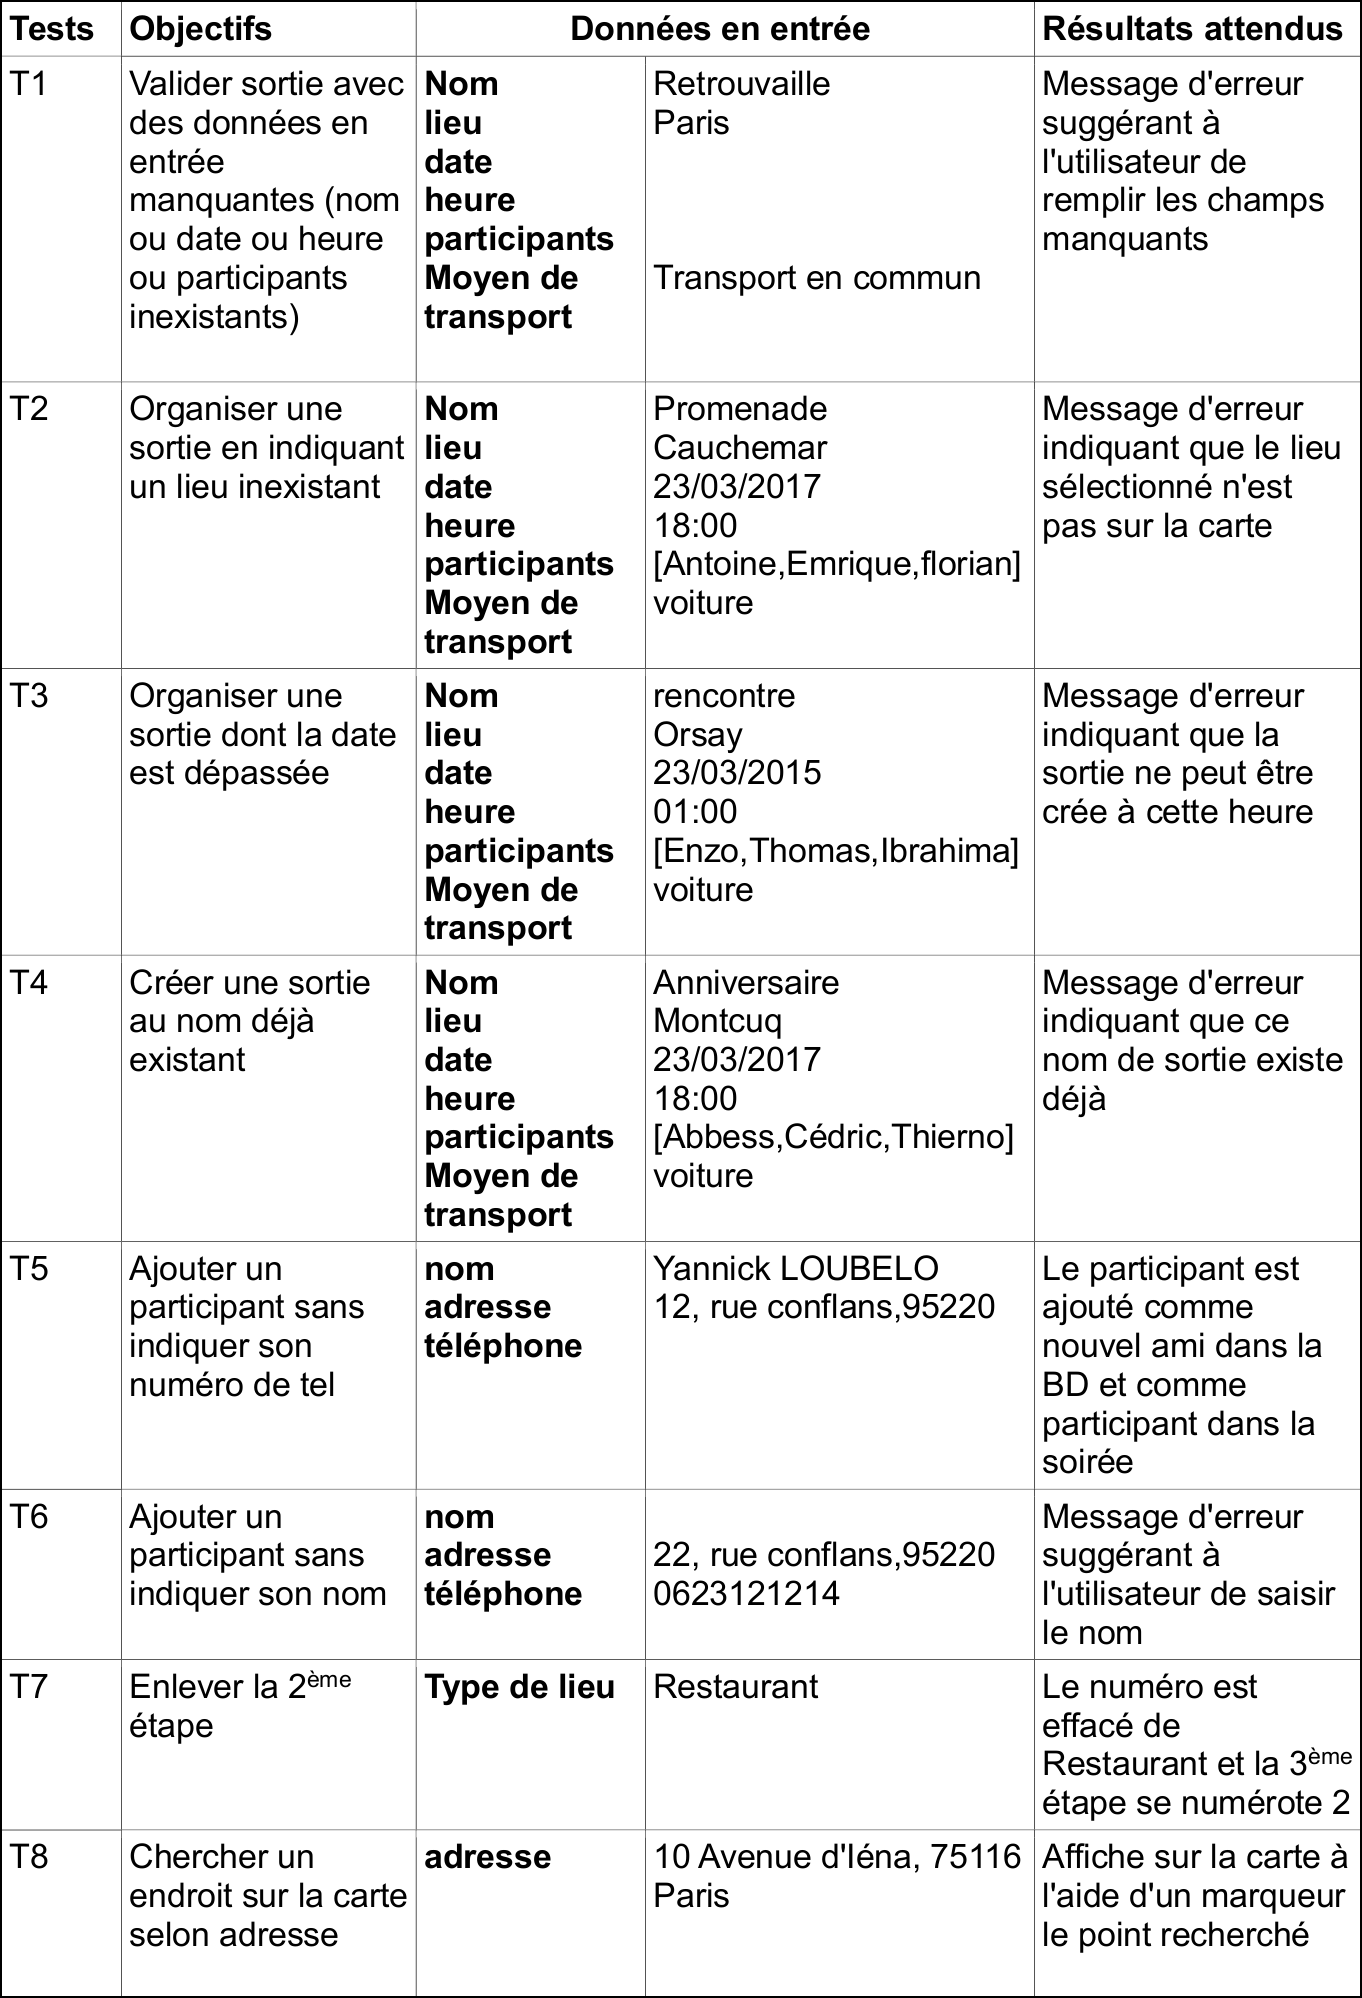
\includegraphics[width=0.97\textwidth]{tests_unitaires_1.png}
\end{figure}
\begin{figure}[!htb]
    \centering
    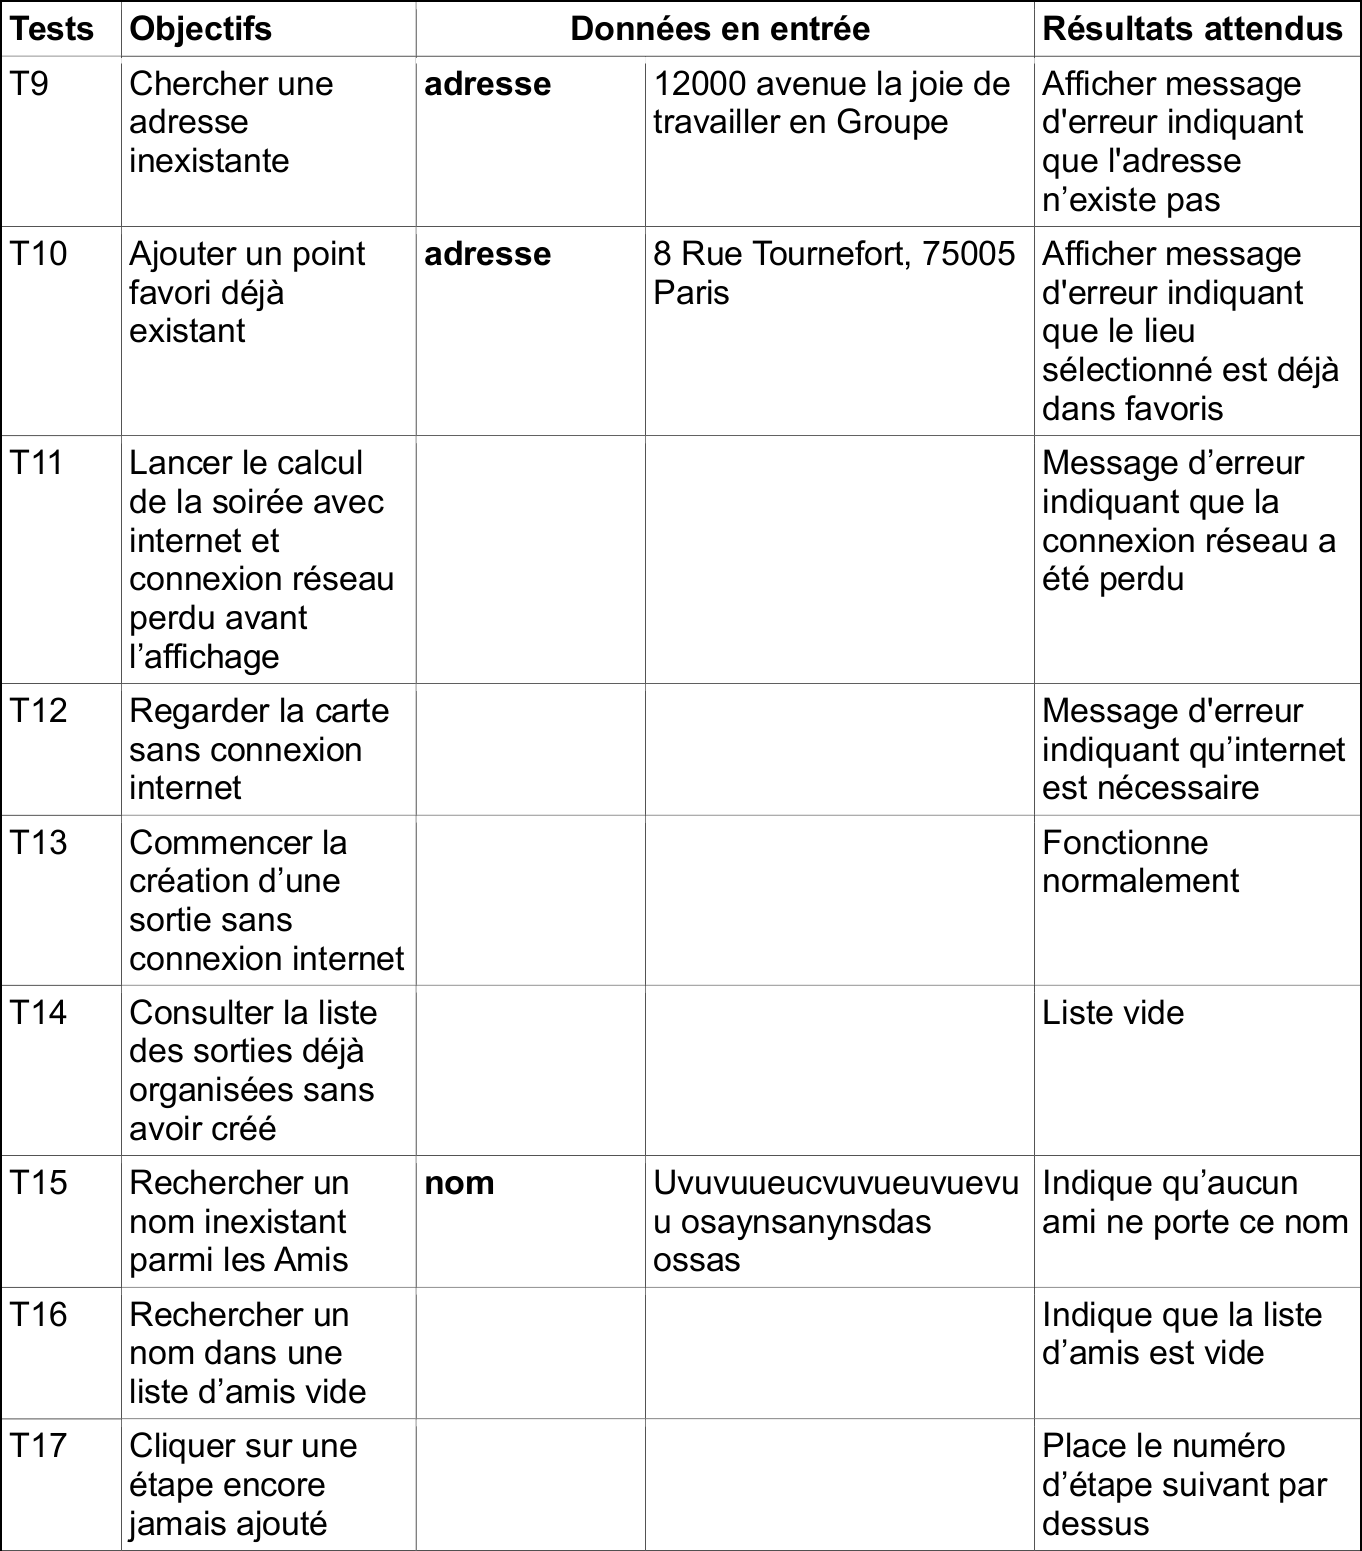
\includegraphics[width=0.97\textwidth]{tests_unitaires_2.png}
\end{figure}
\clearpage

\subsection{Tests fonctionnels}
\begin{figure}[!htb]
    \centering
    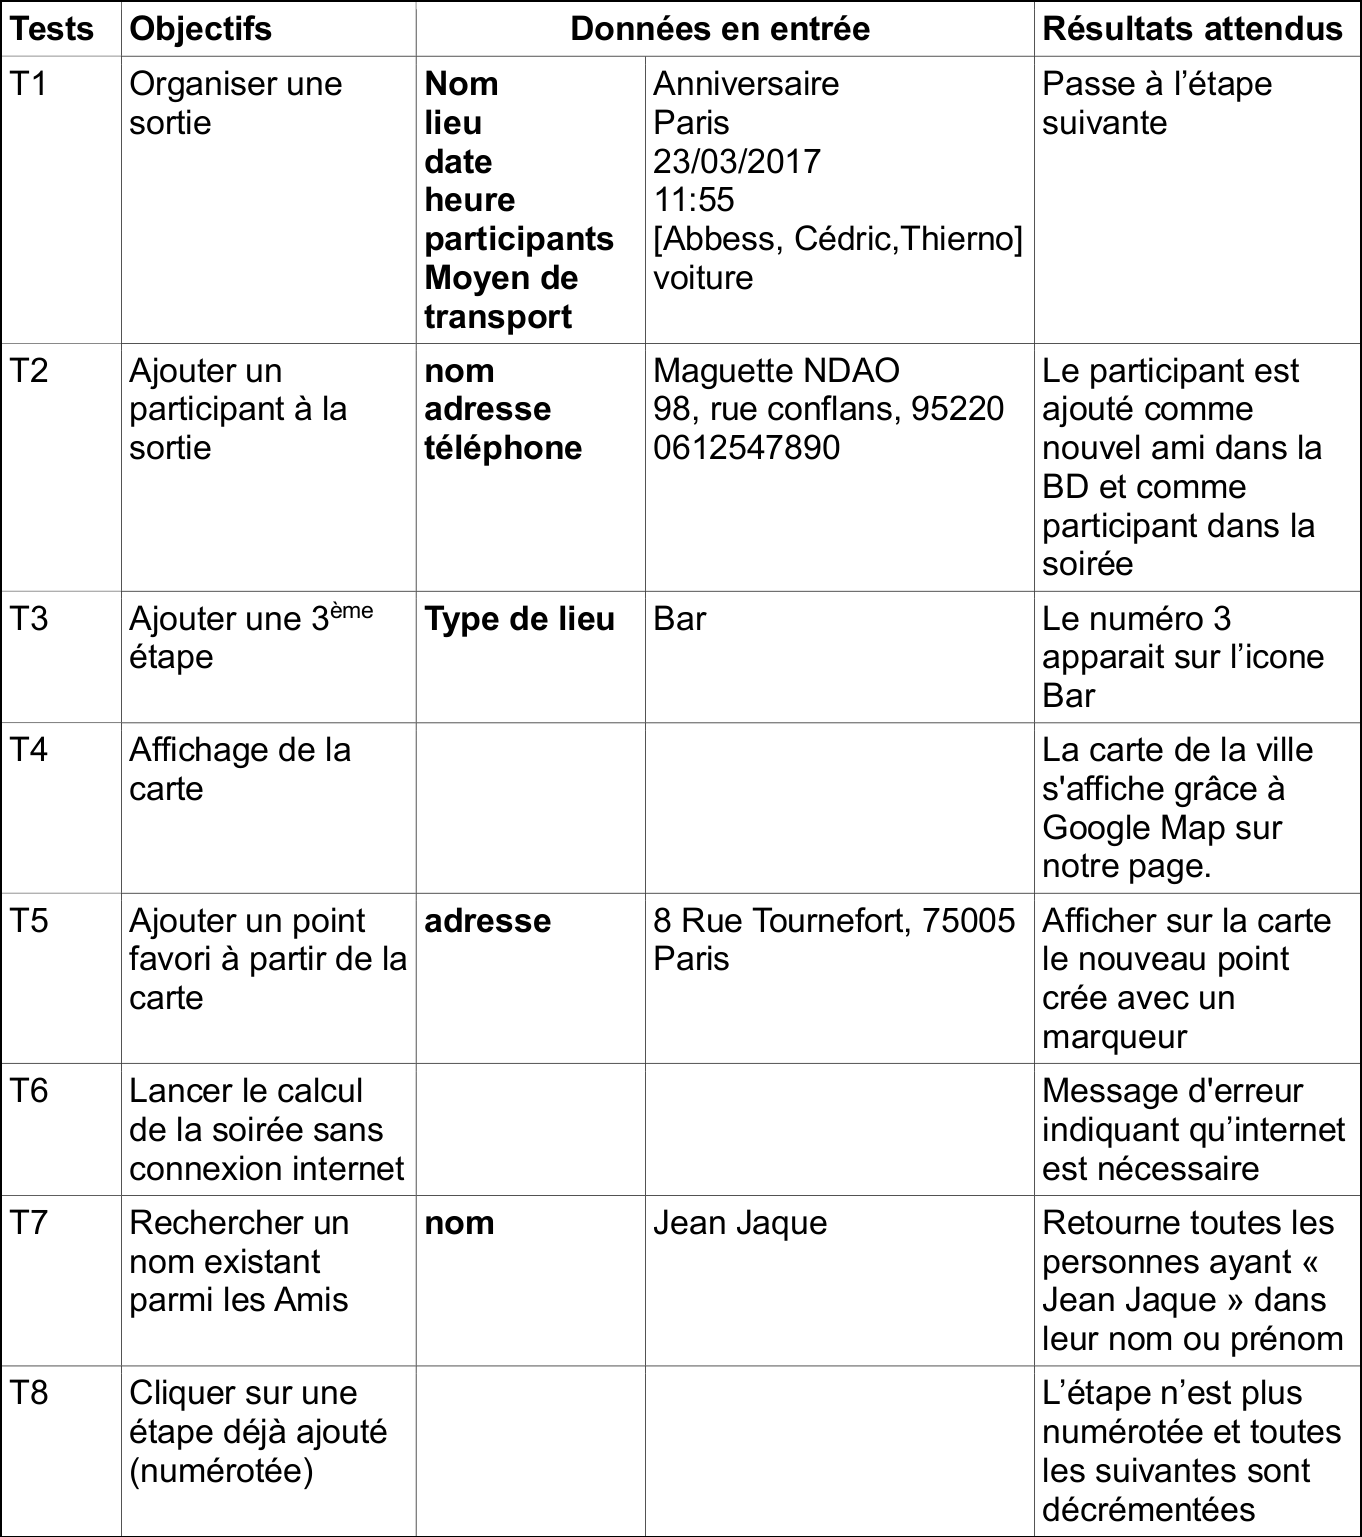
\includegraphics[width=0.97\textwidth]{tests_fonctionels.png}
\end{figure}
\clearpage

\subsection{Tests d’acceptation}
De manière très générale, il faudra que l'application reste fluide en toute condition, ou que les ralentissements soient compréhensibles (calcul en cours, chargement de la carte). De même, les bugs doivent générer des erreurs compréhensibles par l'utilisateur mais en aucun cas un plantage complet pour garantir la robustesse.

Cette application devra aussi respecter les contraintes qui ont été imposées par le cahier des charges. Elle devra donc passer les tests suivants :
\begin{easylist}[itemize] \itemizeTrait
& Essayer de faire fonctionner l'application sans activer internet. Il doit être possible de visualiser les sorties enregistrées (passées ou à venir) et leurs étapes détaillées.
& Que la fonction d’envoi de SMS soit opérationnelle en permettant d'envoyer à tous les participants figurant dans la liste des contacts enregistrés, les informations sur la sortie sélectionnée.
& Que la création de sortie fonctionne de A à Z et que la sortie proposée soit valable en respectant les contraintes et les horaires des lieux de rendez-vous.
& Pourvoir supprimer des Amis et des Favoris de leurs listes respectives.
\end{easylist}

\end{document}